\documentclass[11pt, a4paper]{article}
\usepackage{epsfig}
\usepackage{graphicx}
\usepackage{subfigure}
\usepackage{amssymb, amsmath, amsthm, mathtools}
\usepackage[margin=2.5cm]{geometry}
\usepackage{tikz}
\usepackage{siunitx}
\usepackage{booktabs}
\usepackage{caption}
\usepackage{pgfplots}
\usepackage{listings}
\usepackage{caption}

\makeatletter
\def\fps@figure{hbtp}
\def\fps@table{hbtp}
\makeatother

\let\originalleft\left
\let\originalright\right
\renewcommand{\left}{\mathopen{}\mathclose\bgroup\originalleft}
\renewcommand{\right}{\aftergroup\egroup\originalright}

\lstset{
	breaklines=true,
	postbreak=\mbox{\textcolor{red}{$\hookrightarrow$}\space},
	}

\title{Assignment 4}
\author{Axel Forsman}

\begin{document}
\maketitle

\section{Introduction}

\section{Assignment 1(a)}
\subsection{Problem}
Prove that $\mathbb E[u(t)]$ is maximized as a function of
$\mu$ and $\sigma^2$ when $\mu - k\sigma^2/2$ is maximized.
\subsection{Theory and implementation}
\subsection{Results and discussion}
\begin{align*}
	\mathbb E[u(t)] &= \int_\infty^\infty \frac{1 - e^{-yk}}k \frac1{\sqrt{2\pi\sigma^2}}
		\exp\left(-\frac1{2\sigma^2} (y - \mu)^2\right) \, dy \\
		&= \frac1k \left(\underbrace{\int_\infty^\infty \frac1{\sqrt{2\pi\sigma^2}} \exp\left(-\frac1{2\sigma^2} (y - \mu)^2\right) \, dy}_{=1, \, \text{for integral of pdf of normal distribution}}
		- \int_\infty^\infty e^{-yk} \frac1{\sqrt{2\pi\sigma^2}} \exp\left(-\frac1{2\sigma^2} (y - \mu)^2\right) \, dy\right) \\
		&= \frac1k \left(1 - \int_\infty^\infty \frac1{\sqrt{2\pi\sigma^2}}
			\exp\left(\underbrace{-yk - \frac1{2\sigma^2} (y - \mu)^2}_{\begin{subarray}{1}
				= y^2 - 2y(\mu - \sigma^2k) + \mu^2 \\
				= (y - (\mu - \sigma^2k))^2 + 2\sigma^2k\mu - (\sigma^2k)^2
			\end{subarray}}\right) \, dy\right) \\
		&= \frac1k \left(1 - \exp\left(-\frac{2\sigma^2k\mu - (\sigma^2k)^2}{2\sigma^2}\right)
			\int_\infty^\infty \frac1{\sqrt{2\pi\sigma^2}} \exp\left(-\frac1{2\sigma^2} (y - (\mu - \sigma^2k))^2\right) \, dy\right) \\
		&= \frac1k \left(1 - \exp\left(-k \left(\mu - \frac{k\sigma^2}2\right)\right)\right)
\end{align*}
which is maximized when $\mu - k\sigma^2/2$ is maximized, since
$\left(1 - \exp\left(-k x\right)\right) / k$
is an increasing function of $x$, regardless of $k \ne 0$.

\section{Assignment 1(b)}
\subsection{Problem}
\subsection{Theory and implementation}
\subsection{Results and discussion}
See figure~\ref{fig:stock_weights}.
We see that $w_1$ ratio decreases with $k$
which should imply that \texttt{Comp1} is more instable.
It is also the case that $var(Comp1) > var(Comp2)$.

\begin{figure}
	\centering
	% Created by tikzDevice version 0.12.3 on 2019-10-10 21:33:38
% !TEX encoding = UTF-8 Unicode
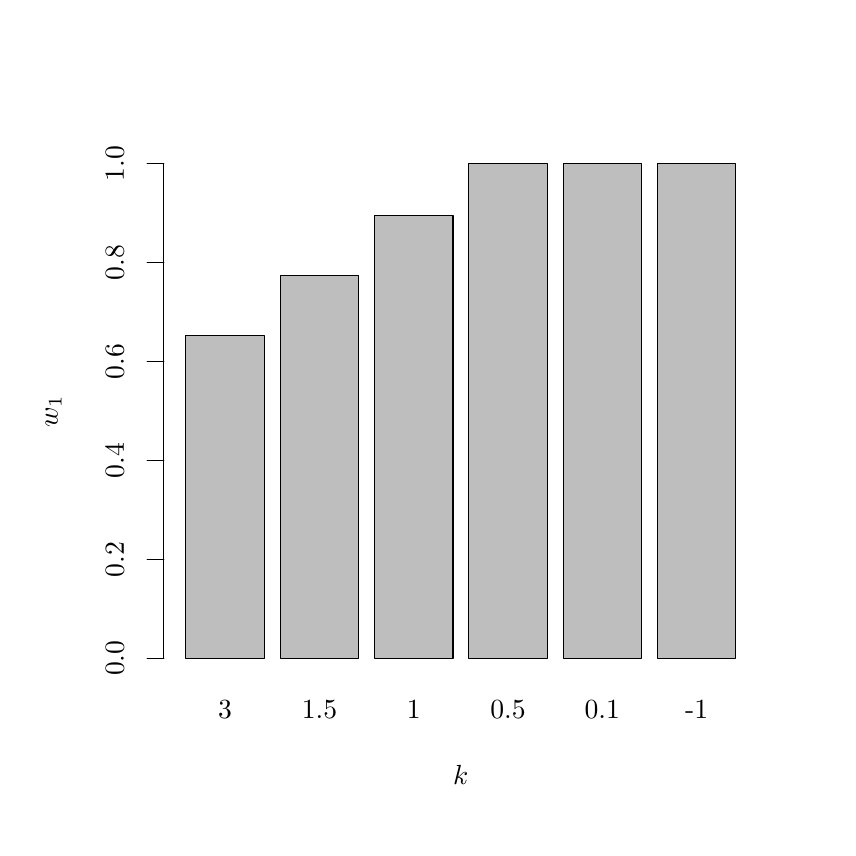
\begin{tikzpicture}[x=1pt,y=1pt]
\definecolor{fillColor}{RGB}{255,255,255}
\path[use as bounding box,fill=fillColor,fill opacity=0.00] (0,0) rectangle (289.08,289.08);
\begin{scope}
\path[clip] (  0.00,  0.00) rectangle (289.08,289.08);
\definecolor{drawColor}{RGB}{0,0,0}
\definecolor{fillColor}{RGB}{190,190,190}

\path[draw=drawColor,line width= 0.4pt,line join=round,line cap=round,fill=fillColor] ( 57.15, 61.20) rectangle ( 85.55,177.81);

\path[draw=drawColor,line width= 0.4pt,line join=round,line cap=round,fill=fillColor] ( 91.23, 61.20) rectangle (119.62,199.53);

\path[draw=drawColor,line width= 0.4pt,line join=round,line cap=round,fill=fillColor] (125.30, 61.20) rectangle (153.70,221.25);

\path[draw=drawColor,line width= 0.4pt,line join=round,line cap=round,fill=fillColor] (159.38, 61.20) rectangle (187.78,239.87);

\path[draw=drawColor,line width= 0.4pt,line join=round,line cap=round,fill=fillColor] (193.46, 61.20) rectangle (221.85,239.87);

\path[draw=drawColor,line width= 0.4pt,line join=round,line cap=round,fill=fillColor] (227.53, 61.20) rectangle (255.93,239.87);
\end{scope}
\begin{scope}
\path[clip] (  0.00,  0.00) rectangle (289.08,289.08);
\definecolor{drawColor}{RGB}{0,0,0}

\node[text=drawColor,anchor=base,inner sep=0pt, outer sep=0pt, scale=  1.00] at ( 71.35, 39.60) {3};

\node[text=drawColor,anchor=base,inner sep=0pt, outer sep=0pt, scale=  1.00] at (105.43, 39.60) {1.5};

\node[text=drawColor,anchor=base,inner sep=0pt, outer sep=0pt, scale=  1.00] at (139.50, 39.60) {1};

\node[text=drawColor,anchor=base,inner sep=0pt, outer sep=0pt, scale=  1.00] at (173.58, 39.60) {0.5};

\node[text=drawColor,anchor=base,inner sep=0pt, outer sep=0pt, scale=  1.00] at (207.65, 39.60) {0.1};

\node[text=drawColor,anchor=base,inner sep=0pt, outer sep=0pt, scale=  1.00] at (241.73, 39.60) {-1};
\end{scope}
\begin{scope}
\path[clip] (  0.00,  0.00) rectangle (289.08,289.08);
\definecolor{drawColor}{RGB}{0,0,0}

\node[text=drawColor,anchor=base,inner sep=0pt, outer sep=0pt, scale=  1.00] at (156.54, 15.60) {$k$};

\node[text=drawColor,rotate= 90.00,anchor=base,inner sep=0pt, outer sep=0pt, scale=  1.00] at ( 10.80,150.54) {$w_1$};
\end{scope}
\begin{scope}
\path[clip] (  0.00,  0.00) rectangle (289.08,289.08);
\definecolor{drawColor}{RGB}{0,0,0}

\path[draw=drawColor,line width= 0.4pt,line join=round,line cap=round] ( 49.20, 61.20) -- ( 49.20,239.88);

\path[draw=drawColor,line width= 0.4pt,line join=round,line cap=round] ( 49.20, 61.20) -- ( 43.20, 61.20);

\path[draw=drawColor,line width= 0.4pt,line join=round,line cap=round] ( 49.20, 96.94) -- ( 43.20, 96.94);

\path[draw=drawColor,line width= 0.4pt,line join=round,line cap=round] ( 49.20,132.67) -- ( 43.20,132.67);

\path[draw=drawColor,line width= 0.4pt,line join=round,line cap=round] ( 49.20,168.41) -- ( 43.20,168.41);

\path[draw=drawColor,line width= 0.4pt,line join=round,line cap=round] ( 49.20,204.14) -- ( 43.20,204.14);

\path[draw=drawColor,line width= 0.4pt,line join=round,line cap=round] ( 49.20,239.88) -- ( 43.20,239.88);

\node[text=drawColor,rotate= 90.00,anchor=base,inner sep=0pt, outer sep=0pt, scale=  1.00] at ( 34.80, 61.20) {0.0};

\node[text=drawColor,rotate= 90.00,anchor=base,inner sep=0pt, outer sep=0pt, scale=  1.00] at ( 34.80, 96.94) {0.2};

\node[text=drawColor,rotate= 90.00,anchor=base,inner sep=0pt, outer sep=0pt, scale=  1.00] at ( 34.80,132.67) {0.4};

\node[text=drawColor,rotate= 90.00,anchor=base,inner sep=0pt, outer sep=0pt, scale=  1.00] at ( 34.80,168.41) {0.6};

\node[text=drawColor,rotate= 90.00,anchor=base,inner sep=0pt, outer sep=0pt, scale=  1.00] at ( 34.80,204.14) {0.8};

\node[text=drawColor,rotate= 90.00,anchor=base,inner sep=0pt, outer sep=0pt, scale=  1.00] at ( 34.80,239.88) {1.0};
\end{scope}
\end{tikzpicture}

	\caption{Plot of the optimized stock weight.
	The ratio that should be invested in \texttt{Comp1} is shown against the value of $k$. \label{fig:stock_weights}}
\end{figure}

\section{Assignment 2(a)}
\subsection{Problem}
Fit a logistic regression to the data, by numerical maximum likelihood
given parameters $a$ and $b$.
\subsection{Theory and implementation}
There are two reports
$$ \text{reports} = \left\{\underbrace{\text{mature}}_1, \underbrace{\text{immature}}_0\right\} $$
Our model is
$$ y \sim Bernoulli(f_1(x)), \quad f_1(x) = \frac{\exp\left(a + b (x - 18)\right)}{1 + \exp\left(a + b (x - 18)\right)} $$
\subsection{Results and discussion}
The fitted logistic regression curve is shown in figure~\ref{fig:logistic_regression}.
We see that the result seems plausible since the curve somewhat mimics the

\begin{figure}
	\centering
	% Created by tikzDevice version 0.12.3 on 2019-10-10 21:36:45
% !TEX encoding = UTF-8 Unicode
\begin{tikzpicture}[x=1pt,y=1pt]
\definecolor{fillColor}{RGB}{255,255,255}
\path[use as bounding box,fill=fillColor,fill opacity=0.00] (0,0) rectangle (289.08,289.08);
\begin{scope}
\path[clip] ( 49.20, 61.20) rectangle (263.88,239.88);
\definecolor{drawColor}{RGB}{0,0,0}

\path[draw=drawColor,line width= 0.4pt,line join=round,line cap=round] ( 57.15, 67.82) --
	( 57.55, 67.83) --
	( 57.95, 67.84) --
	( 58.35, 67.84) --
	( 58.74, 67.85) --
	( 59.14, 67.86) --
	( 59.54, 67.87) --
	( 59.94, 67.89) --
	( 60.34, 67.90) --
	( 60.74, 67.91) --
	( 61.13, 67.92) --
	( 61.53, 67.93) --
	( 61.93, 67.94) --
	( 62.33, 67.95) --
	( 62.73, 67.97) --
	( 63.13, 67.98) --
	( 63.52, 67.99) --
	( 63.92, 68.01) --
	( 64.32, 68.02) --
	( 64.72, 68.04) --
	( 65.12, 68.05) --
	( 65.52, 68.07) --
	( 65.91, 68.08) --
	( 66.31, 68.10) --
	( 66.71, 68.12) --
	( 67.11, 68.13) --
	( 67.51, 68.15) --
	( 67.91, 68.17) --
	( 68.30, 68.19) --
	( 68.70, 68.21) --
	( 69.10, 68.23) --
	( 69.50, 68.25) --
	( 69.90, 68.27) --
	( 70.30, 68.29) --
	( 70.70, 68.32) --
	( 71.09, 68.34) --
	( 71.49, 68.36) --
	( 71.89, 68.39) --
	( 72.29, 68.41) --
	( 72.69, 68.44) --
	( 73.09, 68.47) --
	( 73.48, 68.49) --
	( 73.88, 68.52) --
	( 74.28, 68.55) --
	( 74.68, 68.58) --
	( 75.08, 68.61) --
	( 75.48, 68.64) --
	( 75.87, 68.68) --
	( 76.27, 68.71) --
	( 76.67, 68.74) --
	( 77.07, 68.78) --
	( 77.47, 68.82) --
	( 77.87, 68.85) --
	( 78.26, 68.89) --
	( 78.66, 68.93) --
	( 79.06, 68.97) --
	( 79.46, 69.01) --
	( 79.86, 69.06) --
	( 80.26, 69.10) --
	( 80.65, 69.15) --
	( 81.05, 69.19) --
	( 81.45, 69.24) --
	( 81.85, 69.29) --
	( 82.25, 69.34) --
	( 82.65, 69.40) --
	( 83.04, 69.45) --
	( 83.44, 69.51) --
	( 83.84, 69.56) --
	( 84.24, 69.62) --
	( 84.64, 69.68) --
	( 85.04, 69.75) --
	( 85.43, 69.81) --
	( 85.83, 69.88) --
	( 86.23, 69.94) --
	( 86.63, 70.01) --
	( 87.03, 70.08) --
	( 87.43, 70.16) --
	( 87.82, 70.23) --
	( 88.22, 70.31) --
	( 88.62, 70.39) --
	( 89.02, 70.47) --
	( 89.42, 70.56) --
	( 89.82, 70.64) --
	( 90.21, 70.73) --
	( 90.61, 70.83) --
	( 91.01, 70.92) --
	( 91.41, 71.02) --
	( 91.81, 71.12) --
	( 92.21, 71.22) --
	( 92.60, 71.33) --
	( 93.00, 71.43) --
	( 93.40, 71.54) --
	( 93.80, 71.66) --
	( 94.20, 71.78) --
	( 94.60, 71.90) --
	( 94.99, 72.02) --
	( 95.39, 72.15) --
	( 95.79, 72.28) --
	( 96.19, 72.41) --
	( 96.59, 72.55) --
	( 96.99, 72.69) --
	( 97.38, 72.84) --
	( 97.78, 72.99) --
	( 98.18, 73.14) --
	( 98.58, 73.30) --
	( 98.98, 73.46) --
	( 99.38, 73.63) --
	( 99.77, 73.80) --
	(100.17, 73.98) --
	(100.57, 74.16) --
	(100.97, 74.34) --
	(101.37, 74.53) --
	(101.77, 74.73) --
	(102.16, 74.93) --
	(102.56, 75.14) --
	(102.96, 75.35) --
	(103.36, 75.56) --
	(103.76, 75.79) --
	(104.16, 76.02) --
	(104.56, 76.25) --
	(104.95, 76.49) --
	(105.35, 76.74) --
	(105.75, 76.99) --
	(106.15, 77.25) --
	(106.55, 77.52) --
	(106.95, 77.79) --
	(107.34, 78.07) --
	(107.74, 78.36) --
	(108.14, 78.65) --
	(108.54, 78.95) --
	(108.94, 79.26) --
	(109.34, 79.58) --
	(109.73, 79.90) --
	(110.13, 80.24) --
	(110.53, 80.58) --
	(110.93, 80.93) --
	(111.33, 81.28) --
	(111.73, 81.65) --
	(112.12, 82.03) --
	(112.52, 82.41) --
	(112.92, 82.80) --
	(113.32, 83.21) --
	(113.72, 83.62) --
	(114.12, 84.04) --
	(114.51, 84.47) --
	(114.91, 84.91) --
	(115.31, 85.37) --
	(115.71, 85.83) --
	(116.11, 86.30) --
	(116.51, 86.78) --
	(116.90, 87.28) --
	(117.30, 87.78) --
	(117.70, 88.30) --
	(118.10, 88.83) --
	(118.50, 89.36) --
	(118.90, 89.91) --
	(119.29, 90.48) --
	(119.69, 91.05) --
	(120.09, 91.63) --
	(120.49, 92.23) --
	(120.89, 92.84) --
	(121.29, 93.46) --
	(121.68, 94.10) --
	(122.08, 94.74) --
	(122.48, 95.40) --
	(122.88, 96.07) --
	(123.28, 96.76) --
	(123.68, 97.46) --
	(124.07, 98.17) --
	(124.47, 98.89) --
	(124.87, 99.63) --
	(125.27,100.38) --
	(125.67,101.14) --
	(126.07,101.91) --
	(126.46,102.70) --
	(126.86,103.50) --
	(127.26,104.32) --
	(127.66,105.15) --
	(128.06,105.99) --
	(128.46,106.84) --
	(128.85,107.71) --
	(129.25,108.59) --
	(129.65,109.48) --
	(130.05,110.39) --
	(130.45,111.30) --
	(130.85,112.24) --
	(131.24,113.18) --
	(131.64,114.13) --
	(132.04,115.10) --
	(132.44,116.08) --
	(132.84,117.07) --
	(133.24,118.07) --
	(133.63,119.09) --
	(134.03,120.11) --
	(134.43,121.15) --
	(134.83,122.19) --
	(135.23,123.25) --
	(135.63,124.32) --
	(136.02,125.39) --
	(136.42,126.48) --
	(136.82,127.57) --
	(137.22,128.67) --
	(137.62,129.79) --
	(138.02,130.91) --
	(138.41,132.03) --
	(138.81,133.17) --
	(139.21,134.31) --
	(139.61,135.45) --
	(140.01,136.61) --
	(140.41,137.77) --
	(140.81,138.93) --
	(141.20,140.10) --
	(141.60,141.27) --
	(142.00,142.45) --
	(142.40,143.63) --
	(142.80,144.81) --
	(143.20,145.99) --
	(143.59,147.18) --
	(143.99,148.37) --
	(144.39,149.56) --
	(144.79,150.75) --
	(145.19,151.94) --
	(145.59,153.12) --
	(145.98,154.31) --
	(146.38,155.50) --
	(146.78,156.68) --
	(147.18,157.86) --
	(147.58,159.04) --
	(147.98,160.21) --
	(148.37,161.38) --
	(148.77,162.55) --
	(149.17,163.71) --
	(149.57,164.87) --
	(149.97,166.02) --
	(150.37,167.16) --
	(150.76,168.30) --
	(151.16,169.43) --
	(151.56,170.55) --
	(151.96,171.66) --
	(152.36,172.77) --
	(152.76,173.87) --
	(153.15,174.96) --
	(153.55,176.04) --
	(153.95,177.11) --
	(154.35,178.17) --
	(154.75,179.22) --
	(155.15,180.26) --
	(155.54,181.29) --
	(155.94,182.31) --
	(156.34,183.32) --
	(156.74,184.31) --
	(157.14,185.30) --
	(157.54,186.27) --
	(157.93,187.23) --
	(158.33,188.18) --
	(158.73,189.12) --
	(159.13,190.04) --
	(159.53,190.95) --
	(159.93,191.85) --
	(160.32,192.73) --
	(160.72,193.61) --
	(161.12,194.47) --
	(161.52,195.31) --
	(161.92,196.15) --
	(162.32,196.97) --
	(162.71,197.78) --
	(163.11,198.57) --
	(163.51,199.35) --
	(163.91,200.12) --
	(164.31,200.87) --
	(164.71,201.62) --
	(165.10,202.35) --
	(165.50,203.06) --
	(165.90,203.76) --
	(166.30,204.45) --
	(166.70,205.13) --
	(167.10,205.80) --
	(167.49,206.45) --
	(167.89,207.09) --
	(168.29,207.72) --
	(168.69,208.33) --
	(169.09,208.93) --
	(169.49,209.52) --
	(169.88,210.10) --
	(170.28,210.67) --
	(170.68,211.22) --
	(171.08,211.77) --
	(171.48,212.30) --
	(171.88,212.82) --
	(172.27,213.33) --
	(172.67,213.83) --
	(173.07,214.32) --
	(173.47,214.79) --
	(173.87,215.26) --
	(174.27,215.72) --
	(174.67,216.16) --
	(175.06,216.60) --
	(175.46,217.03) --
	(175.86,217.44) --
	(176.26,217.85) --
	(176.66,218.25) --
	(177.06,218.64) --
	(177.45,219.02) --
	(177.85,219.39) --
	(178.25,219.75) --
	(178.65,220.10) --
	(179.05,220.45) --
	(179.45,220.78) --
	(179.84,221.11) --
	(180.24,221.43) --
	(180.64,221.74) --
	(181.04,222.05) --
	(181.44,222.35) --
	(181.84,222.64) --
	(182.23,222.92) --
	(182.63,223.20) --
	(183.03,223.46) --
	(183.43,223.73) --
	(183.83,223.98) --
	(184.23,224.23) --
	(184.62,224.48) --
	(185.02,224.71) --
	(185.42,224.94) --
	(185.82,225.17) --
	(186.22,225.39) --
	(186.62,225.60) --
	(187.01,225.81) --
	(187.41,226.01) --
	(187.81,226.21) --
	(188.21,226.40) --
	(188.61,226.59) --
	(189.01,226.77) --
	(189.40,226.95) --
	(189.80,227.12) --
	(190.20,227.29) --
	(190.60,227.46) --
	(191.00,227.62) --
	(191.40,227.77) --
	(191.79,227.93) --
	(192.19,228.07) --
	(192.59,228.22) --
	(192.99,228.36) --
	(193.39,228.49) --
	(193.79,228.63) --
	(194.18,228.75) --
	(194.58,228.88) --
	(194.98,229.00) --
	(195.38,229.12) --
	(195.78,229.24) --
	(196.18,229.35) --
	(196.57,229.46) --
	(196.97,229.57) --
	(197.37,229.67) --
	(197.77,229.77) --
	(198.17,229.87) --
	(198.57,229.96) --
	(198.96,230.06) --
	(199.36,230.15) --
	(199.76,230.24) --
	(200.16,230.32) --
	(200.56,230.40) --
	(200.96,230.49) --
	(201.35,230.56) --
	(201.75,230.64) --
	(202.15,230.72) --
	(202.55,230.79) --
	(202.95,230.86) --
	(203.35,230.93) --
	(203.74,230.99) --
	(204.14,231.06) --
	(204.54,231.12) --
	(204.94,231.18) --
	(205.34,231.24) --
	(205.74,231.30) --
	(206.13,231.36) --
	(206.53,231.41) --
	(206.93,231.46) --
	(207.33,231.52) --
	(207.73,231.57) --
	(208.13,231.62) --
	(208.52,231.66) --
	(208.92,231.71) --
	(209.32,231.75) --
	(209.72,231.80) --
	(210.12,231.84) --
	(210.52,231.88) --
	(210.92,231.92) --
	(211.31,231.96) --
	(211.71,232.00) --
	(212.11,232.04) --
	(212.51,232.07) --
	(212.91,232.11) --
	(213.31,232.14) --
	(213.70,232.17) --
	(214.10,232.21) --
	(214.50,232.24) --
	(214.90,232.27) --
	(215.30,232.30) --
	(215.70,232.33) --
	(216.09,232.35) --
	(216.49,232.38) --
	(216.89,232.41) --
	(217.29,232.43) --
	(217.69,232.46) --
	(218.09,232.48) --
	(218.48,232.51) --
	(218.88,232.53) --
	(219.28,232.55) --
	(219.68,232.57) --
	(220.08,232.59) --
	(220.48,232.61) --
	(220.87,232.63) --
	(221.27,232.65) --
	(221.67,232.67) --
	(222.07,232.69) --
	(222.47,232.71) --
	(222.87,232.72) --
	(223.26,232.74) --
	(223.66,232.76) --
	(224.06,232.77) --
	(224.46,232.79) --
	(224.86,232.80) --
	(225.26,232.82) --
	(225.65,232.83) --
	(226.05,232.85) --
	(226.45,232.86) --
	(226.85,232.87) --
	(227.25,232.88) --
	(227.65,232.90) --
	(228.04,232.91) --
	(228.44,232.92) --
	(228.84,232.93) --
	(229.24,232.94) --
	(229.64,232.95) --
	(230.04,232.96) --
	(230.43,232.97) --
	(230.83,232.98) --
	(231.23,232.99) --
	(231.63,233.00) --
	(232.03,233.01) --
	(232.43,233.02) --
	(232.82,233.03) --
	(233.22,233.04) --
	(233.62,233.04) --
	(234.02,233.05) --
	(234.42,233.06) --
	(234.82,233.07) --
	(235.21,233.07) --
	(235.61,233.08) --
	(236.01,233.09) --
	(236.41,233.09) --
	(236.81,233.10) --
	(237.21,233.11) --
	(237.60,233.11) --
	(238.00,233.12) --
	(238.40,233.12) --
	(238.80,233.13) --
	(239.20,233.13) --
	(239.60,233.14) --
	(239.99,233.14) --
	(240.39,233.15) --
	(240.79,233.15) --
	(241.19,233.16) --
	(241.59,233.16) --
	(241.99,233.17) --
	(242.38,233.17) --
	(242.78,233.18) --
	(243.18,233.18) --
	(243.58,233.18) --
	(243.98,233.19) --
	(244.38,233.19) --
	(244.78,233.19) --
	(245.17,233.20) --
	(245.57,233.20) --
	(245.97,233.20) --
	(246.37,233.21) --
	(246.77,233.21) --
	(247.17,233.21) --
	(247.56,233.22) --
	(247.96,233.22) --
	(248.36,233.22) --
	(248.76,233.23) --
	(249.16,233.23) --
	(249.56,233.23) --
	(249.95,233.23) --
	(250.35,233.24) --
	(250.75,233.24) --
	(251.15,233.24) --
	(251.55,233.24) --
	(251.95,233.24) --
	(252.34,233.25) --
	(252.74,233.25) --
	(253.14,233.25) --
	(253.54,233.25) --
	(253.94,233.25) --
	(254.34,233.26) --
	(254.73,233.26) --
	(255.13,233.26) --
	(255.53,233.26) --
	(255.93,233.26);
\end{scope}
\begin{scope}
\path[clip] (  0.00,  0.00) rectangle (289.08,289.08);
\definecolor{drawColor}{RGB}{0,0,0}

\path[draw=drawColor,line width= 0.4pt,line join=round,line cap=round] ( 57.15, 61.20) -- (255.93, 61.20);

\path[draw=drawColor,line width= 0.4pt,line join=round,line cap=round] ( 57.15, 61.20) -- ( 57.15, 55.20);

\path[draw=drawColor,line width= 0.4pt,line join=round,line cap=round] (106.85, 61.20) -- (106.85, 55.20);

\path[draw=drawColor,line width= 0.4pt,line join=round,line cap=round] (156.54, 61.20) -- (156.54, 55.20);

\path[draw=drawColor,line width= 0.4pt,line join=round,line cap=round] (206.23, 61.20) -- (206.23, 55.20);

\path[draw=drawColor,line width= 0.4pt,line join=round,line cap=round] (255.93, 61.20) -- (255.93, 55.20);

\node[text=drawColor,anchor=base,inner sep=0pt, outer sep=0pt, scale=  1.00] at ( 57.15, 39.60) {0};

\node[text=drawColor,anchor=base,inner sep=0pt, outer sep=0pt, scale=  1.00] at (106.85, 39.60) {10};

\node[text=drawColor,anchor=base,inner sep=0pt, outer sep=0pt, scale=  1.00] at (156.54, 39.60) {20};

\node[text=drawColor,anchor=base,inner sep=0pt, outer sep=0pt, scale=  1.00] at (206.23, 39.60) {30};

\node[text=drawColor,anchor=base,inner sep=0pt, outer sep=0pt, scale=  1.00] at (255.93, 39.60) {40};

\path[draw=drawColor,line width= 0.4pt,line join=round,line cap=round] ( 49.20, 67.51) -- ( 49.20,233.32);

\path[draw=drawColor,line width= 0.4pt,line join=round,line cap=round] ( 49.20, 67.51) -- ( 43.20, 67.51);

\path[draw=drawColor,line width= 0.4pt,line join=round,line cap=round] ( 49.20,100.68) -- ( 43.20,100.68);

\path[draw=drawColor,line width= 0.4pt,line join=round,line cap=round] ( 49.20,133.84) -- ( 43.20,133.84);

\path[draw=drawColor,line width= 0.4pt,line join=round,line cap=round] ( 49.20,167.00) -- ( 43.20,167.00);

\path[draw=drawColor,line width= 0.4pt,line join=round,line cap=round] ( 49.20,200.16) -- ( 43.20,200.16);

\path[draw=drawColor,line width= 0.4pt,line join=round,line cap=round] ( 49.20,233.32) -- ( 43.20,233.32);

\node[text=drawColor,rotate= 90.00,anchor=base,inner sep=0pt, outer sep=0pt, scale=  1.00] at ( 34.80, 67.51) {0.0};

\node[text=drawColor,rotate= 90.00,anchor=base,inner sep=0pt, outer sep=0pt, scale=  1.00] at ( 34.80,100.68) {0.2};

\node[text=drawColor,rotate= 90.00,anchor=base,inner sep=0pt, outer sep=0pt, scale=  1.00] at ( 34.80,133.84) {0.4};

\node[text=drawColor,rotate= 90.00,anchor=base,inner sep=0pt, outer sep=0pt, scale=  1.00] at ( 34.80,167.00) {0.6};

\node[text=drawColor,rotate= 90.00,anchor=base,inner sep=0pt, outer sep=0pt, scale=  1.00] at ( 34.80,200.16) {0.8};

\node[text=drawColor,rotate= 90.00,anchor=base,inner sep=0pt, outer sep=0pt, scale=  1.00] at ( 34.80,233.32) {1.0};

\path[draw=drawColor,line width= 0.4pt,line join=round,line cap=round] ( 49.20, 61.20) --
	(263.88, 61.20) --
	(263.88,239.88) --
	( 49.20,239.88) --
	( 49.20, 61.20);
\end{scope}
\begin{scope}
\path[clip] (  0.00,  0.00) rectangle (289.08,289.08);
\definecolor{drawColor}{RGB}{0,0,0}

\node[text=drawColor,anchor=base,inner sep=0pt, outer sep=0pt, scale=  1.00] at (156.54, 15.60) {x};

\path[draw=drawColor,line width= 0.4pt,line join=round,line cap=round] (178.90,233.32) circle (  2.25);

\path[draw=drawColor,line width= 0.4pt,line join=round,line cap=round] (171.45,233.32) circle (  2.25);

\path[draw=drawColor,line width= 0.4pt,line join=round,line cap=round] (164.99,233.32) circle (  2.25);

\path[draw=drawColor,line width= 0.4pt,line join=round,line cap=round] (173.44,233.32) circle (  2.25);

\path[draw=drawColor,line width= 0.4pt,line join=round,line cap=round] (146.10,233.32) circle (  2.25);

\path[draw=drawColor,line width= 0.4pt,line join=round,line cap=round] (171.45,233.32) circle (  2.25);

\path[draw=drawColor,line width= 0.4pt,line join=round,line cap=round] (162.01,233.32) circle (  2.25);

\path[draw=drawColor,line width= 0.4pt,line join=round,line cap=round] (174.43,233.32) circle (  2.25);

\path[draw=drawColor,line width= 0.4pt,line join=round,line cap=round] (152.07,233.32) circle (  2.25);

\path[draw=drawColor,line width= 0.4pt,line join=round,line cap=round] (180.39,233.32) circle (  2.25);

\path[draw=drawColor,line width= 0.4pt,line join=round,line cap=round] (156.04,233.32) circle (  2.25);

\path[draw=drawColor,line width= 0.4pt,line join=round,line cap=round] (154.06,233.32) circle (  2.25);

\path[draw=drawColor,line width= 0.4pt,line join=round,line cap=round] (159.52,233.32) circle (  2.25);

\path[draw=drawColor,line width= 0.4pt,line join=round,line cap=round] (145.11,233.32) circle (  2.25);

\path[draw=drawColor,line width= 0.4pt,line join=round,line cap=round] (171.95,233.32) circle (  2.25);

\path[draw=drawColor,line width= 0.4pt,line join=round,line cap=round] (160.02,233.32) circle (  2.25);

\path[draw=drawColor,line width= 0.4pt,line join=round,line cap=round] (175.42,233.32) circle (  2.25);

\path[draw=drawColor,line width= 0.4pt,line join=round,line cap=round] (177.41,233.32) circle (  2.25);

\path[draw=drawColor,line width= 0.4pt,line join=round,line cap=round] (170.95,233.32) circle (  2.25);

\path[draw=drawColor,line width= 0.4pt,line join=round,line cap=round] (150.58,233.32) circle (  2.25);

\path[draw=drawColor,line width= 0.4pt,line join=round,line cap=round] (174.93,233.32) circle (  2.25);

\path[draw=drawColor,line width= 0.4pt,line join=round,line cap=round] (162.50,233.32) circle (  2.25);

\path[draw=drawColor,line width= 0.4pt,line join=round,line cap=round] (139.15,233.32) circle (  2.25);

\path[draw=drawColor,line width= 0.4pt,line join=round,line cap=round] (172.94,233.32) circle (  2.25);

\path[draw=drawColor,line width= 0.4pt,line join=round,line cap=round] (180.39,233.32) circle (  2.25);

\path[draw=drawColor,line width= 0.4pt,line join=round,line cap=round] (140.14,233.32) circle (  2.25);

\path[draw=drawColor,line width= 0.4pt,line join=round,line cap=round] (146.10,233.32) circle (  2.25);

\path[draw=drawColor,line width= 0.4pt,line join=round,line cap=round] (176.91,233.32) circle (  2.25);

\path[draw=drawColor,line width= 0.4pt,line join=round,line cap=round] (172.44,233.32) circle (  2.25);

\path[draw=drawColor,line width= 0.4pt,line join=round,line cap=round] (172.94,233.32) circle (  2.25);

\path[draw=drawColor,line width= 0.4pt,line join=round,line cap=round] (168.47,233.32) circle (  2.25);

\path[draw=drawColor,line width= 0.4pt,line join=round,line cap=round] (159.52,233.32) circle (  2.25);

\path[draw=drawColor,line width= 0.4pt,line join=round,line cap=round] (143.12,233.32) circle (  2.25);

\path[draw=drawColor,line width= 0.4pt,line join=round,line cap=round] (162.01,233.32) circle (  2.25);

\path[draw=drawColor,line width= 0.4pt,line join=round,line cap=round] (146.60,233.32) circle (  2.25);

\path[draw=drawColor,line width= 0.4pt,line join=round,line cap=round] (157.04,233.32) circle (  2.25);

\path[draw=drawColor,line width= 0.4pt,line join=round,line cap=round] (160.02,233.32) circle (  2.25);

\path[draw=drawColor,line width= 0.4pt,line join=round,line cap=round] (164.99,233.32) circle (  2.25);

\path[draw=drawColor,line width= 0.4pt,line join=round,line cap=round] (166.98,233.32) circle (  2.25);

\path[draw=drawColor,line width= 0.4pt,line join=round,line cap=round] (165.98,233.32) circle (  2.25);

\path[draw=drawColor,line width= 0.4pt,line join=round,line cap=round] (176.91,233.32) circle (  2.25);

\path[draw=drawColor,line width= 0.4pt,line join=round,line cap=round] (164.49,233.32) circle (  2.25);

\path[draw=drawColor,line width= 0.4pt,line join=round,line cap=round] (158.53,233.32) circle (  2.25);

\path[draw=drawColor,line width= 0.4pt,line join=round,line cap=round] (154.55,233.32) circle (  2.25);

\path[draw=drawColor,line width= 0.4pt,line join=round,line cap=round] (151.07,233.32) circle (  2.25);

\path[draw=drawColor,line width= 0.4pt,line join=round,line cap=round] (144.12,233.32) circle (  2.25);

\path[draw=drawColor,line width= 0.4pt,line join=round,line cap=round] (159.52,233.32) circle (  2.25);

\path[draw=drawColor,line width= 0.4pt,line join=round,line cap=round] (153.56,233.32) circle (  2.25);

\path[draw=drawColor,line width= 0.4pt,line join=round,line cap=round] (169.46,233.32) circle (  2.25);

\path[draw=drawColor,line width= 0.4pt,line join=round,line cap=round] (176.91,233.32) circle (  2.25);

\path[draw=drawColor,line width= 0.4pt,line join=round,line cap=round] (122.75, 67.51) circle (  2.25);

\path[draw=drawColor,line width= 0.4pt,line join=round,line cap=round] (131.20, 67.51) circle (  2.25);

\path[draw=drawColor,line width= 0.4pt,line join=round,line cap=round] (130.20, 67.51) circle (  2.25);

\path[draw=drawColor,line width= 0.4pt,line join=round,line cap=round] (123.24, 67.51) circle (  2.25);

\path[draw=drawColor,line width= 0.4pt,line join=round,line cap=round] (144.12, 67.51) circle (  2.25);

\path[draw=drawColor,line width= 0.4pt,line join=round,line cap=round] (126.23, 67.51) circle (  2.25);

\path[draw=drawColor,line width= 0.4pt,line join=round,line cap=round] (137.16, 67.51) circle (  2.25);

\path[draw=drawColor,line width= 0.4pt,line join=round,line cap=round] (126.72, 67.51) circle (  2.25);

\path[draw=drawColor,line width= 0.4pt,line join=round,line cap=round] (126.23, 67.51) circle (  2.25);

\path[draw=drawColor,line width= 0.4pt,line join=round,line cap=round] (127.22, 67.51) circle (  2.25);

\path[draw=drawColor,line width= 0.4pt,line join=round,line cap=round] (130.70, 67.51) circle (  2.25);

\path[draw=drawColor,line width= 0.4pt,line join=round,line cap=round] (132.69, 67.51) circle (  2.25);

\path[draw=drawColor,line width= 0.4pt,line join=round,line cap=round] (120.26, 67.51) circle (  2.25);

\path[draw=drawColor,line width= 0.4pt,line join=round,line cap=round] (130.20, 67.51) circle (  2.25);

\path[draw=drawColor,line width= 0.4pt,line join=round,line cap=round] (138.15, 67.51) circle (  2.25);

\path[draw=drawColor,line width= 0.4pt,line join=round,line cap=round] (117.78, 67.51) circle (  2.25);

\path[draw=drawColor,line width= 0.4pt,line join=round,line cap=round] (118.77, 67.51) circle (  2.25);

\path[draw=drawColor,line width= 0.4pt,line join=round,line cap=round] (130.20, 67.51) circle (  2.25);

\path[draw=drawColor,line width= 0.4pt,line join=round,line cap=round] (135.17, 67.51) circle (  2.25);

\path[draw=drawColor,line width= 0.4pt,line join=round,line cap=round] (129.70, 67.51) circle (  2.25);

\path[draw=drawColor,line width= 0.4pt,line join=round,line cap=round] (131.20, 67.51) circle (  2.25);

\path[draw=drawColor,line width= 0.4pt,line join=round,line cap=round] (141.13, 67.51) circle (  2.25);

\path[draw=drawColor,line width= 0.4pt,line join=round,line cap=round] (140.64, 67.51) circle (  2.25);

\path[draw=drawColor,line width= 0.4pt,line join=round,line cap=round] (135.67, 67.51) circle (  2.25);

\path[draw=drawColor,line width= 0.4pt,line join=round,line cap=round] (134.67, 67.51) circle (  2.25);

\path[draw=drawColor,line width= 0.4pt,line join=round,line cap=round] (137.66, 67.51) circle (  2.25);

\path[draw=drawColor,line width= 0.4pt,line join=round,line cap=round] (140.14, 67.51) circle (  2.25);

\path[draw=drawColor,line width= 0.4pt,line join=round,line cap=round] (117.28, 67.51) circle (  2.25);

\path[draw=drawColor,line width= 0.4pt,line join=round,line cap=round] (139.64, 67.51) circle (  2.25);

\path[draw=drawColor,line width= 0.4pt,line join=round,line cap=round] (130.20, 67.51) circle (  2.25);

\path[draw=drawColor,line width= 0.4pt,line join=round,line cap=round] (129.21, 67.51) circle (  2.25);

\path[draw=drawColor,line width= 0.4pt,line join=round,line cap=round] (136.66, 67.51) circle (  2.25);

\path[draw=drawColor,line width= 0.4pt,line join=round,line cap=round] (152.07, 67.51) circle (  2.25);

\path[draw=drawColor,line width= 0.4pt,line join=round,line cap=round] (125.73, 67.51) circle (  2.25);

\path[draw=drawColor,line width= 0.4pt,line join=round,line cap=round] (120.26, 67.51) circle (  2.25);

\path[draw=drawColor,line width= 0.4pt,line join=round,line cap=round] (145.61, 67.51) circle (  2.25);

\path[draw=drawColor,line width= 0.4pt,line join=round,line cap=round] (141.63, 67.51) circle (  2.25);

\path[draw=drawColor,line width= 0.4pt,line join=round,line cap=round] (130.70, 67.51) circle (  2.25);

\path[draw=drawColor,line width= 0.4pt,line join=round,line cap=round] (132.19, 67.51) circle (  2.25);

\path[draw=drawColor,line width= 0.4pt,line join=round,line cap=round] (118.28, 67.51) circle (  2.25);

\path[draw=drawColor,line width= 0.4pt,line join=round,line cap=round] (131.69, 67.51) circle (  2.25);

\path[draw=drawColor,line width= 0.4pt,line join=round,line cap=round] (135.67, 67.51) circle (  2.25);

\path[draw=drawColor,line width= 0.4pt,line join=round,line cap=round] (142.13, 67.51) circle (  2.25);

\path[draw=drawColor,line width= 0.4pt,line join=round,line cap=round] (118.28, 67.51) circle (  2.25);

\path[draw=drawColor,line width= 0.4pt,line join=round,line cap=round] (140.64, 67.51) circle (  2.25);

\path[draw=drawColor,line width= 0.4pt,line join=round,line cap=round] (119.77, 67.51) circle (  2.25);

\path[draw=drawColor,line width= 0.4pt,line join=round,line cap=round] (123.74, 67.51) circle (  2.25);

\path[draw=drawColor,line width= 0.4pt,line join=round,line cap=round] (134.67, 67.51) circle (  2.25);

\path[draw=drawColor,line width= 0.4pt,line join=round,line cap=round] (139.64, 67.51) circle (  2.25);

\path[draw=drawColor,line width= 0.4pt,line join=round,line cap=round] (146.10, 67.51) circle (  2.25);
\end{scope}
\end{tikzpicture}

	\caption{Plot of the data together with the obtained logistic regression curve. \label{fig:logistic_regression}}
\end{figure}

\section{Assignment 2(b)}
\subsection{Problem}
\subsection{Theory and implementation}
\subsection{Results and discussion}

\begin{figure}
	\centering
	% Created by tikzDevice version 0.12.3 on 2019-10-10 21:56:19
% !TEX encoding = UTF-8 Unicode
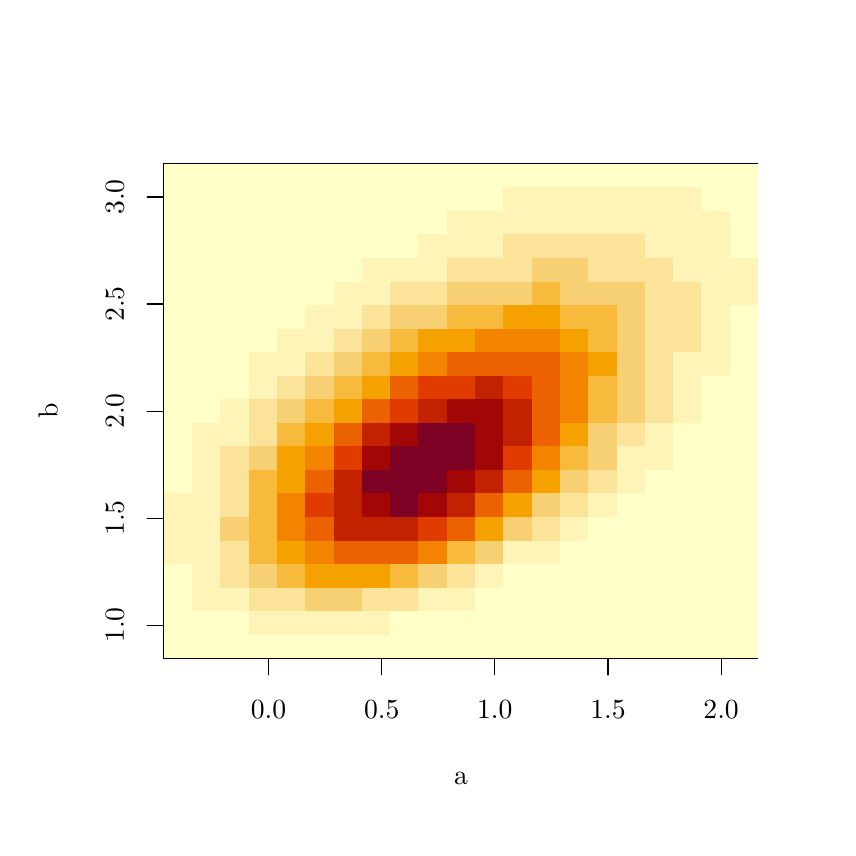
\begin{tikzpicture}[x=1pt,y=1pt]
\definecolor{fillColor}{RGB}{255,255,255}
\path[use as bounding box,fill=fillColor,fill opacity=0.00] (0,0) rectangle (289.08,289.08);
\begin{scope}
\path[clip] (  0.00,  0.00) rectangle (289.08,289.08);
\definecolor{drawColor}{RGB}{0,0,0}

\path[draw=drawColor,line width= 0.4pt,line join=round,line cap=round] ( 87.02, 61.20) -- (250.59, 61.20);

\path[draw=drawColor,line width= 0.4pt,line join=round,line cap=round] ( 87.02, 61.20) -- ( 87.02, 55.20);

\path[draw=drawColor,line width= 0.4pt,line join=round,line cap=round] (127.92, 61.20) -- (127.92, 55.20);

\path[draw=drawColor,line width= 0.4pt,line join=round,line cap=round] (168.81, 61.20) -- (168.81, 55.20);

\path[draw=drawColor,line width= 0.4pt,line join=round,line cap=round] (209.70, 61.20) -- (209.70, 55.20);

\path[draw=drawColor,line width= 0.4pt,line join=round,line cap=round] (250.59, 61.20) -- (250.59, 55.20);

\node[text=drawColor,anchor=base,inner sep=0pt, outer sep=0pt, scale=  1.00] at ( 87.02, 39.60) {0.0};

\node[text=drawColor,anchor=base,inner sep=0pt, outer sep=0pt, scale=  1.00] at (127.92, 39.60) {0.5};

\node[text=drawColor,anchor=base,inner sep=0pt, outer sep=0pt, scale=  1.00] at (168.81, 39.60) {1.0};

\node[text=drawColor,anchor=base,inner sep=0pt, outer sep=0pt, scale=  1.00] at (209.70, 39.60) {1.5};

\node[text=drawColor,anchor=base,inner sep=0pt, outer sep=0pt, scale=  1.00] at (250.59, 39.60) {2.0};

\path[draw=drawColor,line width= 0.4pt,line join=round,line cap=round] ( 49.20, 73.19) -- ( 49.20,227.89);

\path[draw=drawColor,line width= 0.4pt,line join=round,line cap=round] ( 49.20, 73.19) -- ( 43.20, 73.19);

\path[draw=drawColor,line width= 0.4pt,line join=round,line cap=round] ( 49.20,111.86) -- ( 43.20,111.86);

\path[draw=drawColor,line width= 0.4pt,line join=round,line cap=round] ( 49.20,150.54) -- ( 43.20,150.54);

\path[draw=drawColor,line width= 0.4pt,line join=round,line cap=round] ( 49.20,189.22) -- ( 43.20,189.22);

\path[draw=drawColor,line width= 0.4pt,line join=round,line cap=round] ( 49.20,227.89) -- ( 43.20,227.89);

\node[text=drawColor,rotate= 90.00,anchor=base,inner sep=0pt, outer sep=0pt, scale=  1.00] at ( 34.80, 73.19) {1.0};

\node[text=drawColor,rotate= 90.00,anchor=base,inner sep=0pt, outer sep=0pt, scale=  1.00] at ( 34.80,111.86) {1.5};

\node[text=drawColor,rotate= 90.00,anchor=base,inner sep=0pt, outer sep=0pt, scale=  1.00] at ( 34.80,150.54) {2.0};

\node[text=drawColor,rotate= 90.00,anchor=base,inner sep=0pt, outer sep=0pt, scale=  1.00] at ( 34.80,189.22) {2.5};

\node[text=drawColor,rotate= 90.00,anchor=base,inner sep=0pt, outer sep=0pt, scale=  1.00] at ( 34.80,227.89) {3.0};

\path[draw=drawColor,line width= 0.4pt,line join=round,line cap=round] ( 49.20, 61.20) --
	(263.88, 61.20) --
	(263.88,239.88) --
	( 49.20,239.88) --
	( 49.20, 61.20);
\end{scope}
\begin{scope}
\path[clip] (  0.00,  0.00) rectangle (289.08,289.08);
\definecolor{drawColor}{RGB}{0,0,0}

\node[text=drawColor,anchor=base,inner sep=0pt, outer sep=0pt, scale=  1.00] at (156.54, 15.60) {a};

\node[text=drawColor,rotate= 90.00,anchor=base,inner sep=0pt, outer sep=0pt, scale=  1.00] at ( 10.80,150.54) {b};
\end{scope}
\begin{scope}
\path[clip] ( 49.20, 61.20) rectangle (263.88,239.88);
\definecolor{fillColor}{RGB}{255,255,200}

\path[fill=fillColor] ( 49.20, 61.20) rectangle ( 59.42, 69.71);

\path[fill=fillColor] ( 49.20, 69.71) rectangle ( 59.42, 78.22);

\path[fill=fillColor] ( 49.20, 78.22) rectangle ( 59.42, 86.73);

\path[fill=fillColor] ( 49.20, 86.73) rectangle ( 59.42, 95.23);
\definecolor{fillColor}{RGB}{255,244,183}

\path[fill=fillColor] ( 49.20, 95.23) rectangle ( 59.42,103.74);

\path[fill=fillColor] ( 49.20,103.74) rectangle ( 59.42,112.25);

\path[fill=fillColor] ( 49.20,112.25) rectangle ( 59.42,120.76);
\definecolor{fillColor}{RGB}{255,255,200}

\path[fill=fillColor] ( 49.20,120.76) rectangle ( 59.42,129.27);

\path[fill=fillColor] ( 49.20,129.27) rectangle ( 59.42,137.78);

\path[fill=fillColor] ( 49.20,137.78) rectangle ( 59.42,146.29);

\path[fill=fillColor] ( 49.20,146.29) rectangle ( 59.42,154.79);

\path[fill=fillColor] ( 49.20,154.79) rectangle ( 59.42,163.30);

\path[fill=fillColor] ( 49.20,163.30) rectangle ( 59.42,171.81);

\path[fill=fillColor] ( 49.20,171.81) rectangle ( 59.42,180.32);

\path[fill=fillColor] ( 49.20,180.32) rectangle ( 59.42,188.83);

\path[fill=fillColor] ( 49.20,188.83) rectangle ( 59.42,197.34);

\path[fill=fillColor] ( 49.20,197.34) rectangle ( 59.42,205.85);

\path[fill=fillColor] ( 49.20,205.85) rectangle ( 59.42,214.35);

\path[fill=fillColor] ( 49.20,214.35) rectangle ( 59.42,222.86);

\path[fill=fillColor] ( 49.20,222.86) rectangle ( 59.42,231.37);

\path[fill=fillColor] ( 49.20,231.37) rectangle ( 59.42,239.88);

\path[fill=fillColor] ( 59.42, 61.20) rectangle ( 69.65, 69.71);

\path[fill=fillColor] ( 59.42, 69.71) rectangle ( 69.65, 78.22);
\definecolor{fillColor}{RGB}{255,244,183}

\path[fill=fillColor] ( 59.42, 78.22) rectangle ( 69.65, 86.73);

\path[fill=fillColor] ( 59.42, 86.73) rectangle ( 69.65, 95.23);

\path[fill=fillColor] ( 59.42, 95.23) rectangle ( 69.65,103.74);

\path[fill=fillColor] ( 59.42,103.74) rectangle ( 69.65,112.25);

\path[fill=fillColor] ( 59.42,112.25) rectangle ( 69.65,120.76);

\path[fill=fillColor] ( 59.42,120.76) rectangle ( 69.65,129.27);

\path[fill=fillColor] ( 59.42,129.27) rectangle ( 69.65,137.78);

\path[fill=fillColor] ( 59.42,137.78) rectangle ( 69.65,146.29);
\definecolor{fillColor}{RGB}{255,255,200}

\path[fill=fillColor] ( 59.42,146.29) rectangle ( 69.65,154.79);

\path[fill=fillColor] ( 59.42,154.79) rectangle ( 69.65,163.30);

\path[fill=fillColor] ( 59.42,163.30) rectangle ( 69.65,171.81);

\path[fill=fillColor] ( 59.42,171.81) rectangle ( 69.65,180.32);

\path[fill=fillColor] ( 59.42,180.32) rectangle ( 69.65,188.83);

\path[fill=fillColor] ( 59.42,188.83) rectangle ( 69.65,197.34);

\path[fill=fillColor] ( 59.42,197.34) rectangle ( 69.65,205.85);

\path[fill=fillColor] ( 59.42,205.85) rectangle ( 69.65,214.35);

\path[fill=fillColor] ( 59.42,214.35) rectangle ( 69.65,222.86);

\path[fill=fillColor] ( 59.42,222.86) rectangle ( 69.65,231.37);

\path[fill=fillColor] ( 59.42,231.37) rectangle ( 69.65,239.88);

\path[fill=fillColor] ( 69.65, 61.20) rectangle ( 79.87, 69.71);

\path[fill=fillColor] ( 69.65, 69.71) rectangle ( 79.87, 78.22);
\definecolor{fillColor}{RGB}{255,244,183}

\path[fill=fillColor] ( 69.65, 78.22) rectangle ( 79.87, 86.73);
\definecolor{fillColor}{RGB}{251,228,154}

\path[fill=fillColor] ( 69.65, 86.73) rectangle ( 79.87, 95.23);

\path[fill=fillColor] ( 69.65, 95.23) rectangle ( 79.87,103.74);
\definecolor{fillColor}{RGB}{248,208,116}

\path[fill=fillColor] ( 69.65,103.74) rectangle ( 79.87,112.25);
\definecolor{fillColor}{RGB}{251,228,154}

\path[fill=fillColor] ( 69.65,112.25) rectangle ( 79.87,120.76);

\path[fill=fillColor] ( 69.65,120.76) rectangle ( 79.87,129.27);

\path[fill=fillColor] ( 69.65,129.27) rectangle ( 79.87,137.78);
\definecolor{fillColor}{RGB}{255,244,183}

\path[fill=fillColor] ( 69.65,137.78) rectangle ( 79.87,146.29);

\path[fill=fillColor] ( 69.65,146.29) rectangle ( 79.87,154.79);
\definecolor{fillColor}{RGB}{255,255,200}

\path[fill=fillColor] ( 69.65,154.79) rectangle ( 79.87,163.30);

\path[fill=fillColor] ( 69.65,163.30) rectangle ( 79.87,171.81);

\path[fill=fillColor] ( 69.65,171.81) rectangle ( 79.87,180.32);

\path[fill=fillColor] ( 69.65,180.32) rectangle ( 79.87,188.83);

\path[fill=fillColor] ( 69.65,188.83) rectangle ( 79.87,197.34);

\path[fill=fillColor] ( 69.65,197.34) rectangle ( 79.87,205.85);

\path[fill=fillColor] ( 69.65,205.85) rectangle ( 79.87,214.35);

\path[fill=fillColor] ( 69.65,214.35) rectangle ( 79.87,222.86);

\path[fill=fillColor] ( 69.65,222.86) rectangle ( 79.87,231.37);

\path[fill=fillColor] ( 69.65,231.37) rectangle ( 79.87,239.88);

\path[fill=fillColor] ( 79.87, 61.20) rectangle ( 90.09, 69.71);
\definecolor{fillColor}{RGB}{255,244,183}

\path[fill=fillColor] ( 79.87, 69.71) rectangle ( 90.09, 78.22);
\definecolor{fillColor}{RGB}{251,228,154}

\path[fill=fillColor] ( 79.87, 78.22) rectangle ( 90.09, 86.73);
\definecolor{fillColor}{RGB}{248,208,116}

\path[fill=fillColor] ( 79.87, 86.73) rectangle ( 90.09, 95.23);
\definecolor{fillColor}{RGB}{247,186,60}

\path[fill=fillColor] ( 79.87, 95.23) rectangle ( 90.09,103.74);

\path[fill=fillColor] ( 79.87,103.74) rectangle ( 90.09,112.25);

\path[fill=fillColor] ( 79.87,112.25) rectangle ( 90.09,120.76);

\path[fill=fillColor] ( 79.87,120.76) rectangle ( 90.09,129.27);
\definecolor{fillColor}{RGB}{248,208,116}

\path[fill=fillColor] ( 79.87,129.27) rectangle ( 90.09,137.78);
\definecolor{fillColor}{RGB}{251,228,154}

\path[fill=fillColor] ( 79.87,137.78) rectangle ( 90.09,146.29);

\path[fill=fillColor] ( 79.87,146.29) rectangle ( 90.09,154.79);
\definecolor{fillColor}{RGB}{255,244,183}

\path[fill=fillColor] ( 79.87,154.79) rectangle ( 90.09,163.30);

\path[fill=fillColor] ( 79.87,163.30) rectangle ( 90.09,171.81);
\definecolor{fillColor}{RGB}{255,255,200}

\path[fill=fillColor] ( 79.87,171.81) rectangle ( 90.09,180.32);

\path[fill=fillColor] ( 79.87,180.32) rectangle ( 90.09,188.83);

\path[fill=fillColor] ( 79.87,188.83) rectangle ( 90.09,197.34);

\path[fill=fillColor] ( 79.87,197.34) rectangle ( 90.09,205.85);

\path[fill=fillColor] ( 79.87,205.85) rectangle ( 90.09,214.35);

\path[fill=fillColor] ( 79.87,214.35) rectangle ( 90.09,222.86);

\path[fill=fillColor] ( 79.87,222.86) rectangle ( 90.09,231.37);

\path[fill=fillColor] ( 79.87,231.37) rectangle ( 90.09,239.88);

\path[fill=fillColor] ( 90.09, 61.20) rectangle (100.31, 69.71);
\definecolor{fillColor}{RGB}{255,244,183}

\path[fill=fillColor] ( 90.09, 69.71) rectangle (100.31, 78.22);
\definecolor{fillColor}{RGB}{251,228,154}

\path[fill=fillColor] ( 90.09, 78.22) rectangle (100.31, 86.73);
\definecolor{fillColor}{RGB}{247,186,60}

\path[fill=fillColor] ( 90.09, 86.73) rectangle (100.31, 95.23);
\definecolor{fillColor}{RGB}{245,161,0}

\path[fill=fillColor] ( 90.09, 95.23) rectangle (100.31,103.74);
\definecolor{fillColor}{RGB}{242,132,0}

\path[fill=fillColor] ( 90.09,103.74) rectangle (100.31,112.25);

\path[fill=fillColor] ( 90.09,112.25) rectangle (100.31,120.76);
\definecolor{fillColor}{RGB}{245,161,0}

\path[fill=fillColor] ( 90.09,120.76) rectangle (100.31,129.27);

\path[fill=fillColor] ( 90.09,129.27) rectangle (100.31,137.78);
\definecolor{fillColor}{RGB}{247,186,60}

\path[fill=fillColor] ( 90.09,137.78) rectangle (100.31,146.29);
\definecolor{fillColor}{RGB}{248,208,116}

\path[fill=fillColor] ( 90.09,146.29) rectangle (100.31,154.79);
\definecolor{fillColor}{RGB}{251,228,154}

\path[fill=fillColor] ( 90.09,154.79) rectangle (100.31,163.30);
\definecolor{fillColor}{RGB}{255,244,183}

\path[fill=fillColor] ( 90.09,163.30) rectangle (100.31,171.81);

\path[fill=fillColor] ( 90.09,171.81) rectangle (100.31,180.32);
\definecolor{fillColor}{RGB}{255,255,200}

\path[fill=fillColor] ( 90.09,180.32) rectangle (100.31,188.83);

\path[fill=fillColor] ( 90.09,188.83) rectangle (100.31,197.34);

\path[fill=fillColor] ( 90.09,197.34) rectangle (100.31,205.85);

\path[fill=fillColor] ( 90.09,205.85) rectangle (100.31,214.35);

\path[fill=fillColor] ( 90.09,214.35) rectangle (100.31,222.86);

\path[fill=fillColor] ( 90.09,222.86) rectangle (100.31,231.37);

\path[fill=fillColor] ( 90.09,231.37) rectangle (100.31,239.88);

\path[fill=fillColor] (100.31, 61.20) rectangle (110.54, 69.71);
\definecolor{fillColor}{RGB}{255,244,183}

\path[fill=fillColor] (100.31, 69.71) rectangle (110.54, 78.22);
\definecolor{fillColor}{RGB}{248,208,116}

\path[fill=fillColor] (100.31, 78.22) rectangle (110.54, 86.73);
\definecolor{fillColor}{RGB}{245,161,0}

\path[fill=fillColor] (100.31, 86.73) rectangle (110.54, 95.23);
\definecolor{fillColor}{RGB}{242,132,0}

\path[fill=fillColor] (100.31, 95.23) rectangle (110.54,103.74);
\definecolor{fillColor}{RGB}{237,98,0}

\path[fill=fillColor] (100.31,103.74) rectangle (110.54,112.25);
\definecolor{fillColor}{RGB}{225,60,0}

\path[fill=fillColor] (100.31,112.25) rectangle (110.54,120.76);
\definecolor{fillColor}{RGB}{237,98,0}

\path[fill=fillColor] (100.31,120.76) rectangle (110.54,129.27);
\definecolor{fillColor}{RGB}{242,132,0}

\path[fill=fillColor] (100.31,129.27) rectangle (110.54,137.78);
\definecolor{fillColor}{RGB}{245,161,0}

\path[fill=fillColor] (100.31,137.78) rectangle (110.54,146.29);
\definecolor{fillColor}{RGB}{247,186,60}

\path[fill=fillColor] (100.31,146.29) rectangle (110.54,154.79);
\definecolor{fillColor}{RGB}{248,208,116}

\path[fill=fillColor] (100.31,154.79) rectangle (110.54,163.30);
\definecolor{fillColor}{RGB}{251,228,154}

\path[fill=fillColor] (100.31,163.30) rectangle (110.54,171.81);
\definecolor{fillColor}{RGB}{255,244,183}

\path[fill=fillColor] (100.31,171.81) rectangle (110.54,180.32);

\path[fill=fillColor] (100.31,180.32) rectangle (110.54,188.83);
\definecolor{fillColor}{RGB}{255,255,200}

\path[fill=fillColor] (100.31,188.83) rectangle (110.54,197.34);

\path[fill=fillColor] (100.31,197.34) rectangle (110.54,205.85);

\path[fill=fillColor] (100.31,205.85) rectangle (110.54,214.35);

\path[fill=fillColor] (100.31,214.35) rectangle (110.54,222.86);

\path[fill=fillColor] (100.31,222.86) rectangle (110.54,231.37);

\path[fill=fillColor] (100.31,231.37) rectangle (110.54,239.88);

\path[fill=fillColor] (110.54, 61.20) rectangle (120.76, 69.71);
\definecolor{fillColor}{RGB}{255,244,183}

\path[fill=fillColor] (110.54, 69.71) rectangle (120.76, 78.22);
\definecolor{fillColor}{RGB}{248,208,116}

\path[fill=fillColor] (110.54, 78.22) rectangle (120.76, 86.73);
\definecolor{fillColor}{RGB}{245,161,0}

\path[fill=fillColor] (110.54, 86.73) rectangle (120.76, 95.23);
\definecolor{fillColor}{RGB}{237,98,0}

\path[fill=fillColor] (110.54, 95.23) rectangle (120.76,103.74);
\definecolor{fillColor}{RGB}{195,34,0}

\path[fill=fillColor] (110.54,103.74) rectangle (120.76,112.25);

\path[fill=fillColor] (110.54,112.25) rectangle (120.76,120.76);

\path[fill=fillColor] (110.54,120.76) rectangle (120.76,129.27);
\definecolor{fillColor}{RGB}{225,60,0}

\path[fill=fillColor] (110.54,129.27) rectangle (120.76,137.78);
\definecolor{fillColor}{RGB}{237,98,0}

\path[fill=fillColor] (110.54,137.78) rectangle (120.76,146.29);
\definecolor{fillColor}{RGB}{245,161,0}

\path[fill=fillColor] (110.54,146.29) rectangle (120.76,154.79);
\definecolor{fillColor}{RGB}{247,186,60}

\path[fill=fillColor] (110.54,154.79) rectangle (120.76,163.30);
\definecolor{fillColor}{RGB}{248,208,116}

\path[fill=fillColor] (110.54,163.30) rectangle (120.76,171.81);
\definecolor{fillColor}{RGB}{251,228,154}

\path[fill=fillColor] (110.54,171.81) rectangle (120.76,180.32);
\definecolor{fillColor}{RGB}{255,244,183}

\path[fill=fillColor] (110.54,180.32) rectangle (120.76,188.83);

\path[fill=fillColor] (110.54,188.83) rectangle (120.76,197.34);
\definecolor{fillColor}{RGB}{255,255,200}

\path[fill=fillColor] (110.54,197.34) rectangle (120.76,205.85);

\path[fill=fillColor] (110.54,205.85) rectangle (120.76,214.35);

\path[fill=fillColor] (110.54,214.35) rectangle (120.76,222.86);

\path[fill=fillColor] (110.54,222.86) rectangle (120.76,231.37);

\path[fill=fillColor] (110.54,231.37) rectangle (120.76,239.88);

\path[fill=fillColor] (120.76, 61.20) rectangle (130.98, 69.71);
\definecolor{fillColor}{RGB}{255,244,183}

\path[fill=fillColor] (120.76, 69.71) rectangle (130.98, 78.22);
\definecolor{fillColor}{RGB}{251,228,154}

\path[fill=fillColor] (120.76, 78.22) rectangle (130.98, 86.73);
\definecolor{fillColor}{RGB}{245,161,0}

\path[fill=fillColor] (120.76, 86.73) rectangle (130.98, 95.23);
\definecolor{fillColor}{RGB}{237,98,0}

\path[fill=fillColor] (120.76, 95.23) rectangle (130.98,103.74);
\definecolor{fillColor}{RGB}{195,34,0}

\path[fill=fillColor] (120.76,103.74) rectangle (130.98,112.25);
\definecolor{fillColor}{RGB}{162,7,6}

\path[fill=fillColor] (120.76,112.25) rectangle (130.98,120.76);
\definecolor{fillColor}{RGB}{125,0,37}

\path[fill=fillColor] (120.76,120.76) rectangle (130.98,129.27);
\definecolor{fillColor}{RGB}{162,7,6}

\path[fill=fillColor] (120.76,129.27) rectangle (130.98,137.78);
\definecolor{fillColor}{RGB}{195,34,0}

\path[fill=fillColor] (120.76,137.78) rectangle (130.98,146.29);
\definecolor{fillColor}{RGB}{237,98,0}

\path[fill=fillColor] (120.76,146.29) rectangle (130.98,154.79);
\definecolor{fillColor}{RGB}{245,161,0}

\path[fill=fillColor] (120.76,154.79) rectangle (130.98,163.30);
\definecolor{fillColor}{RGB}{247,186,60}

\path[fill=fillColor] (120.76,163.30) rectangle (130.98,171.81);
\definecolor{fillColor}{RGB}{248,208,116}

\path[fill=fillColor] (120.76,171.81) rectangle (130.98,180.32);
\definecolor{fillColor}{RGB}{251,228,154}

\path[fill=fillColor] (120.76,180.32) rectangle (130.98,188.83);
\definecolor{fillColor}{RGB}{255,244,183}

\path[fill=fillColor] (120.76,188.83) rectangle (130.98,197.34);

\path[fill=fillColor] (120.76,197.34) rectangle (130.98,205.85);
\definecolor{fillColor}{RGB}{255,255,200}

\path[fill=fillColor] (120.76,205.85) rectangle (130.98,214.35);

\path[fill=fillColor] (120.76,214.35) rectangle (130.98,222.86);

\path[fill=fillColor] (120.76,222.86) rectangle (130.98,231.37);

\path[fill=fillColor] (120.76,231.37) rectangle (130.98,239.88);

\path[fill=fillColor] (130.98, 61.20) rectangle (141.21, 69.71);

\path[fill=fillColor] (130.98, 69.71) rectangle (141.21, 78.22);
\definecolor{fillColor}{RGB}{251,228,154}

\path[fill=fillColor] (130.98, 78.22) rectangle (141.21, 86.73);
\definecolor{fillColor}{RGB}{247,186,60}

\path[fill=fillColor] (130.98, 86.73) rectangle (141.21, 95.23);
\definecolor{fillColor}{RGB}{237,98,0}

\path[fill=fillColor] (130.98, 95.23) rectangle (141.21,103.74);
\definecolor{fillColor}{RGB}{195,34,0}

\path[fill=fillColor] (130.98,103.74) rectangle (141.21,112.25);
\definecolor{fillColor}{RGB}{125,0,37}

\path[fill=fillColor] (130.98,112.25) rectangle (141.21,120.76);

\path[fill=fillColor] (130.98,120.76) rectangle (141.21,129.27);

\path[fill=fillColor] (130.98,129.27) rectangle (141.21,137.78);
\definecolor{fillColor}{RGB}{162,7,6}

\path[fill=fillColor] (130.98,137.78) rectangle (141.21,146.29);
\definecolor{fillColor}{RGB}{225,60,0}

\path[fill=fillColor] (130.98,146.29) rectangle (141.21,154.79);
\definecolor{fillColor}{RGB}{237,98,0}

\path[fill=fillColor] (130.98,154.79) rectangle (141.21,163.30);
\definecolor{fillColor}{RGB}{245,161,0}

\path[fill=fillColor] (130.98,163.30) rectangle (141.21,171.81);
\definecolor{fillColor}{RGB}{247,186,60}

\path[fill=fillColor] (130.98,171.81) rectangle (141.21,180.32);
\definecolor{fillColor}{RGB}{248,208,116}

\path[fill=fillColor] (130.98,180.32) rectangle (141.21,188.83);
\definecolor{fillColor}{RGB}{251,228,154}

\path[fill=fillColor] (130.98,188.83) rectangle (141.21,197.34);
\definecolor{fillColor}{RGB}{255,244,183}

\path[fill=fillColor] (130.98,197.34) rectangle (141.21,205.85);
\definecolor{fillColor}{RGB}{255,255,200}

\path[fill=fillColor] (130.98,205.85) rectangle (141.21,214.35);

\path[fill=fillColor] (130.98,214.35) rectangle (141.21,222.86);

\path[fill=fillColor] (130.98,222.86) rectangle (141.21,231.37);

\path[fill=fillColor] (130.98,231.37) rectangle (141.21,239.88);

\path[fill=fillColor] (141.21, 61.20) rectangle (151.43, 69.71);

\path[fill=fillColor] (141.21, 69.71) rectangle (151.43, 78.22);
\definecolor{fillColor}{RGB}{255,244,183}

\path[fill=fillColor] (141.21, 78.22) rectangle (151.43, 86.73);
\definecolor{fillColor}{RGB}{248,208,116}

\path[fill=fillColor] (141.21, 86.73) rectangle (151.43, 95.23);
\definecolor{fillColor}{RGB}{242,132,0}

\path[fill=fillColor] (141.21, 95.23) rectangle (151.43,103.74);
\definecolor{fillColor}{RGB}{225,60,0}

\path[fill=fillColor] (141.21,103.74) rectangle (151.43,112.25);
\definecolor{fillColor}{RGB}{162,7,6}

\path[fill=fillColor] (141.21,112.25) rectangle (151.43,120.76);
\definecolor{fillColor}{RGB}{125,0,37}

\path[fill=fillColor] (141.21,120.76) rectangle (151.43,129.27);

\path[fill=fillColor] (141.21,129.27) rectangle (151.43,137.78);

\path[fill=fillColor] (141.21,137.78) rectangle (151.43,146.29);
\definecolor{fillColor}{RGB}{195,34,0}

\path[fill=fillColor] (141.21,146.29) rectangle (151.43,154.79);
\definecolor{fillColor}{RGB}{225,60,0}

\path[fill=fillColor] (141.21,154.79) rectangle (151.43,163.30);
\definecolor{fillColor}{RGB}{242,132,0}

\path[fill=fillColor] (141.21,163.30) rectangle (151.43,171.81);
\definecolor{fillColor}{RGB}{245,161,0}

\path[fill=fillColor] (141.21,171.81) rectangle (151.43,180.32);
\definecolor{fillColor}{RGB}{248,208,116}

\path[fill=fillColor] (141.21,180.32) rectangle (151.43,188.83);
\definecolor{fillColor}{RGB}{251,228,154}

\path[fill=fillColor] (141.21,188.83) rectangle (151.43,197.34);
\definecolor{fillColor}{RGB}{255,244,183}

\path[fill=fillColor] (141.21,197.34) rectangle (151.43,205.85);

\path[fill=fillColor] (141.21,205.85) rectangle (151.43,214.35);
\definecolor{fillColor}{RGB}{255,255,200}

\path[fill=fillColor] (141.21,214.35) rectangle (151.43,222.86);

\path[fill=fillColor] (141.21,222.86) rectangle (151.43,231.37);

\path[fill=fillColor] (141.21,231.37) rectangle (151.43,239.88);

\path[fill=fillColor] (151.43, 61.20) rectangle (161.65, 69.71);

\path[fill=fillColor] (151.43, 69.71) rectangle (161.65, 78.22);
\definecolor{fillColor}{RGB}{255,244,183}

\path[fill=fillColor] (151.43, 78.22) rectangle (161.65, 86.73);
\definecolor{fillColor}{RGB}{251,228,154}

\path[fill=fillColor] (151.43, 86.73) rectangle (161.65, 95.23);
\definecolor{fillColor}{RGB}{247,186,60}

\path[fill=fillColor] (151.43, 95.23) rectangle (161.65,103.74);
\definecolor{fillColor}{RGB}{237,98,0}

\path[fill=fillColor] (151.43,103.74) rectangle (161.65,112.25);
\definecolor{fillColor}{RGB}{195,34,0}

\path[fill=fillColor] (151.43,112.25) rectangle (161.65,120.76);
\definecolor{fillColor}{RGB}{162,7,6}

\path[fill=fillColor] (151.43,120.76) rectangle (161.65,129.27);
\definecolor{fillColor}{RGB}{125,0,37}

\path[fill=fillColor] (151.43,129.27) rectangle (161.65,137.78);

\path[fill=fillColor] (151.43,137.78) rectangle (161.65,146.29);
\definecolor{fillColor}{RGB}{162,7,6}

\path[fill=fillColor] (151.43,146.29) rectangle (161.65,154.79);
\definecolor{fillColor}{RGB}{225,60,0}

\path[fill=fillColor] (151.43,154.79) rectangle (161.65,163.30);
\definecolor{fillColor}{RGB}{237,98,0}

\path[fill=fillColor] (151.43,163.30) rectangle (161.65,171.81);
\definecolor{fillColor}{RGB}{245,161,0}

\path[fill=fillColor] (151.43,171.81) rectangle (161.65,180.32);
\definecolor{fillColor}{RGB}{247,186,60}

\path[fill=fillColor] (151.43,180.32) rectangle (161.65,188.83);
\definecolor{fillColor}{RGB}{248,208,116}

\path[fill=fillColor] (151.43,188.83) rectangle (161.65,197.34);
\definecolor{fillColor}{RGB}{251,228,154}

\path[fill=fillColor] (151.43,197.34) rectangle (161.65,205.85);
\definecolor{fillColor}{RGB}{255,244,183}

\path[fill=fillColor] (151.43,205.85) rectangle (161.65,214.35);

\path[fill=fillColor] (151.43,214.35) rectangle (161.65,222.86);
\definecolor{fillColor}{RGB}{255,255,200}

\path[fill=fillColor] (151.43,222.86) rectangle (161.65,231.37);

\path[fill=fillColor] (151.43,231.37) rectangle (161.65,239.88);

\path[fill=fillColor] (161.65, 61.20) rectangle (171.87, 69.71);

\path[fill=fillColor] (161.65, 69.71) rectangle (171.87, 78.22);

\path[fill=fillColor] (161.65, 78.22) rectangle (171.87, 86.73);
\definecolor{fillColor}{RGB}{255,244,183}

\path[fill=fillColor] (161.65, 86.73) rectangle (171.87, 95.23);
\definecolor{fillColor}{RGB}{248,208,116}

\path[fill=fillColor] (161.65, 95.23) rectangle (171.87,103.74);
\definecolor{fillColor}{RGB}{245,161,0}

\path[fill=fillColor] (161.65,103.74) rectangle (171.87,112.25);
\definecolor{fillColor}{RGB}{237,98,0}

\path[fill=fillColor] (161.65,112.25) rectangle (171.87,120.76);
\definecolor{fillColor}{RGB}{195,34,0}

\path[fill=fillColor] (161.65,120.76) rectangle (171.87,129.27);
\definecolor{fillColor}{RGB}{162,7,6}

\path[fill=fillColor] (161.65,129.27) rectangle (171.87,137.78);

\path[fill=fillColor] (161.65,137.78) rectangle (171.87,146.29);

\path[fill=fillColor] (161.65,146.29) rectangle (171.87,154.79);
\definecolor{fillColor}{RGB}{195,34,0}

\path[fill=fillColor] (161.65,154.79) rectangle (171.87,163.30);
\definecolor{fillColor}{RGB}{237,98,0}

\path[fill=fillColor] (161.65,163.30) rectangle (171.87,171.81);
\definecolor{fillColor}{RGB}{242,132,0}

\path[fill=fillColor] (161.65,171.81) rectangle (171.87,180.32);
\definecolor{fillColor}{RGB}{247,186,60}

\path[fill=fillColor] (161.65,180.32) rectangle (171.87,188.83);
\definecolor{fillColor}{RGB}{248,208,116}

\path[fill=fillColor] (161.65,188.83) rectangle (171.87,197.34);
\definecolor{fillColor}{RGB}{251,228,154}

\path[fill=fillColor] (161.65,197.34) rectangle (171.87,205.85);
\definecolor{fillColor}{RGB}{255,244,183}

\path[fill=fillColor] (161.65,205.85) rectangle (171.87,214.35);

\path[fill=fillColor] (161.65,214.35) rectangle (171.87,222.86);
\definecolor{fillColor}{RGB}{255,255,200}

\path[fill=fillColor] (161.65,222.86) rectangle (171.87,231.37);

\path[fill=fillColor] (161.65,231.37) rectangle (171.87,239.88);

\path[fill=fillColor] (171.87, 61.20) rectangle (182.10, 69.71);

\path[fill=fillColor] (171.87, 69.71) rectangle (182.10, 78.22);

\path[fill=fillColor] (171.87, 78.22) rectangle (182.10, 86.73);

\path[fill=fillColor] (171.87, 86.73) rectangle (182.10, 95.23);
\definecolor{fillColor}{RGB}{255,244,183}

\path[fill=fillColor] (171.87, 95.23) rectangle (182.10,103.74);
\definecolor{fillColor}{RGB}{248,208,116}

\path[fill=fillColor] (171.87,103.74) rectangle (182.10,112.25);
\definecolor{fillColor}{RGB}{245,161,0}

\path[fill=fillColor] (171.87,112.25) rectangle (182.10,120.76);
\definecolor{fillColor}{RGB}{237,98,0}

\path[fill=fillColor] (171.87,120.76) rectangle (182.10,129.27);
\definecolor{fillColor}{RGB}{225,60,0}

\path[fill=fillColor] (171.87,129.27) rectangle (182.10,137.78);
\definecolor{fillColor}{RGB}{195,34,0}

\path[fill=fillColor] (171.87,137.78) rectangle (182.10,146.29);

\path[fill=fillColor] (171.87,146.29) rectangle (182.10,154.79);
\definecolor{fillColor}{RGB}{225,60,0}

\path[fill=fillColor] (171.87,154.79) rectangle (182.10,163.30);
\definecolor{fillColor}{RGB}{237,98,0}

\path[fill=fillColor] (171.87,163.30) rectangle (182.10,171.81);
\definecolor{fillColor}{RGB}{242,132,0}

\path[fill=fillColor] (171.87,171.81) rectangle (182.10,180.32);
\definecolor{fillColor}{RGB}{245,161,0}

\path[fill=fillColor] (171.87,180.32) rectangle (182.10,188.83);
\definecolor{fillColor}{RGB}{248,208,116}

\path[fill=fillColor] (171.87,188.83) rectangle (182.10,197.34);
\definecolor{fillColor}{RGB}{251,228,154}

\path[fill=fillColor] (171.87,197.34) rectangle (182.10,205.85);

\path[fill=fillColor] (171.87,205.85) rectangle (182.10,214.35);
\definecolor{fillColor}{RGB}{255,244,183}

\path[fill=fillColor] (171.87,214.35) rectangle (182.10,222.86);

\path[fill=fillColor] (171.87,222.86) rectangle (182.10,231.37);
\definecolor{fillColor}{RGB}{255,255,200}

\path[fill=fillColor] (171.87,231.37) rectangle (182.10,239.88);

\path[fill=fillColor] (182.10, 61.20) rectangle (192.32, 69.71);

\path[fill=fillColor] (182.10, 69.71) rectangle (192.32, 78.22);

\path[fill=fillColor] (182.10, 78.22) rectangle (192.32, 86.73);

\path[fill=fillColor] (182.10, 86.73) rectangle (192.32, 95.23);
\definecolor{fillColor}{RGB}{255,244,183}

\path[fill=fillColor] (182.10, 95.23) rectangle (192.32,103.74);
\definecolor{fillColor}{RGB}{251,228,154}

\path[fill=fillColor] (182.10,103.74) rectangle (192.32,112.25);
\definecolor{fillColor}{RGB}{248,208,116}

\path[fill=fillColor] (182.10,112.25) rectangle (192.32,120.76);
\definecolor{fillColor}{RGB}{245,161,0}

\path[fill=fillColor] (182.10,120.76) rectangle (192.32,129.27);
\definecolor{fillColor}{RGB}{242,132,0}

\path[fill=fillColor] (182.10,129.27) rectangle (192.32,137.78);
\definecolor{fillColor}{RGB}{237,98,0}

\path[fill=fillColor] (182.10,137.78) rectangle (192.32,146.29);

\path[fill=fillColor] (182.10,146.29) rectangle (192.32,154.79);

\path[fill=fillColor] (182.10,154.79) rectangle (192.32,163.30);

\path[fill=fillColor] (182.10,163.30) rectangle (192.32,171.81);
\definecolor{fillColor}{RGB}{242,132,0}

\path[fill=fillColor] (182.10,171.81) rectangle (192.32,180.32);
\definecolor{fillColor}{RGB}{245,161,0}

\path[fill=fillColor] (182.10,180.32) rectangle (192.32,188.83);
\definecolor{fillColor}{RGB}{247,186,60}

\path[fill=fillColor] (182.10,188.83) rectangle (192.32,197.34);
\definecolor{fillColor}{RGB}{248,208,116}

\path[fill=fillColor] (182.10,197.34) rectangle (192.32,205.85);
\definecolor{fillColor}{RGB}{251,228,154}

\path[fill=fillColor] (182.10,205.85) rectangle (192.32,214.35);
\definecolor{fillColor}{RGB}{255,244,183}

\path[fill=fillColor] (182.10,214.35) rectangle (192.32,222.86);

\path[fill=fillColor] (182.10,222.86) rectangle (192.32,231.37);
\definecolor{fillColor}{RGB}{255,255,200}

\path[fill=fillColor] (182.10,231.37) rectangle (192.32,239.88);

\path[fill=fillColor] (192.32, 61.20) rectangle (202.54, 69.71);

\path[fill=fillColor] (192.32, 69.71) rectangle (202.54, 78.22);

\path[fill=fillColor] (192.32, 78.22) rectangle (202.54, 86.73);

\path[fill=fillColor] (192.32, 86.73) rectangle (202.54, 95.23);

\path[fill=fillColor] (192.32, 95.23) rectangle (202.54,103.74);
\definecolor{fillColor}{RGB}{255,244,183}

\path[fill=fillColor] (192.32,103.74) rectangle (202.54,112.25);
\definecolor{fillColor}{RGB}{251,228,154}

\path[fill=fillColor] (192.32,112.25) rectangle (202.54,120.76);
\definecolor{fillColor}{RGB}{248,208,116}

\path[fill=fillColor] (192.32,120.76) rectangle (202.54,129.27);
\definecolor{fillColor}{RGB}{247,186,60}

\path[fill=fillColor] (192.32,129.27) rectangle (202.54,137.78);
\definecolor{fillColor}{RGB}{245,161,0}

\path[fill=fillColor] (192.32,137.78) rectangle (202.54,146.29);
\definecolor{fillColor}{RGB}{242,132,0}

\path[fill=fillColor] (192.32,146.29) rectangle (202.54,154.79);

\path[fill=fillColor] (192.32,154.79) rectangle (202.54,163.30);

\path[fill=fillColor] (192.32,163.30) rectangle (202.54,171.81);
\definecolor{fillColor}{RGB}{245,161,0}

\path[fill=fillColor] (192.32,171.81) rectangle (202.54,180.32);
\definecolor{fillColor}{RGB}{247,186,60}

\path[fill=fillColor] (192.32,180.32) rectangle (202.54,188.83);
\definecolor{fillColor}{RGB}{248,208,116}

\path[fill=fillColor] (192.32,188.83) rectangle (202.54,197.34);

\path[fill=fillColor] (192.32,197.34) rectangle (202.54,205.85);
\definecolor{fillColor}{RGB}{251,228,154}

\path[fill=fillColor] (192.32,205.85) rectangle (202.54,214.35);
\definecolor{fillColor}{RGB}{255,244,183}

\path[fill=fillColor] (192.32,214.35) rectangle (202.54,222.86);

\path[fill=fillColor] (192.32,222.86) rectangle (202.54,231.37);
\definecolor{fillColor}{RGB}{255,255,200}

\path[fill=fillColor] (192.32,231.37) rectangle (202.54,239.88);

\path[fill=fillColor] (202.54, 61.20) rectangle (212.77, 69.71);

\path[fill=fillColor] (202.54, 69.71) rectangle (212.77, 78.22);

\path[fill=fillColor] (202.54, 78.22) rectangle (212.77, 86.73);

\path[fill=fillColor] (202.54, 86.73) rectangle (212.77, 95.23);

\path[fill=fillColor] (202.54, 95.23) rectangle (212.77,103.74);

\path[fill=fillColor] (202.54,103.74) rectangle (212.77,112.25);
\definecolor{fillColor}{RGB}{255,244,183}

\path[fill=fillColor] (202.54,112.25) rectangle (212.77,120.76);
\definecolor{fillColor}{RGB}{251,228,154}

\path[fill=fillColor] (202.54,120.76) rectangle (212.77,129.27);
\definecolor{fillColor}{RGB}{248,208,116}

\path[fill=fillColor] (202.54,129.27) rectangle (212.77,137.78);

\path[fill=fillColor] (202.54,137.78) rectangle (212.77,146.29);
\definecolor{fillColor}{RGB}{247,186,60}

\path[fill=fillColor] (202.54,146.29) rectangle (212.77,154.79);

\path[fill=fillColor] (202.54,154.79) rectangle (212.77,163.30);
\definecolor{fillColor}{RGB}{245,161,0}

\path[fill=fillColor] (202.54,163.30) rectangle (212.77,171.81);
\definecolor{fillColor}{RGB}{247,186,60}

\path[fill=fillColor] (202.54,171.81) rectangle (212.77,180.32);

\path[fill=fillColor] (202.54,180.32) rectangle (212.77,188.83);
\definecolor{fillColor}{RGB}{248,208,116}

\path[fill=fillColor] (202.54,188.83) rectangle (212.77,197.34);
\definecolor{fillColor}{RGB}{251,228,154}

\path[fill=fillColor] (202.54,197.34) rectangle (212.77,205.85);

\path[fill=fillColor] (202.54,205.85) rectangle (212.77,214.35);
\definecolor{fillColor}{RGB}{255,244,183}

\path[fill=fillColor] (202.54,214.35) rectangle (212.77,222.86);

\path[fill=fillColor] (202.54,222.86) rectangle (212.77,231.37);
\definecolor{fillColor}{RGB}{255,255,200}

\path[fill=fillColor] (202.54,231.37) rectangle (212.77,239.88);

\path[fill=fillColor] (212.77, 61.20) rectangle (222.99, 69.71);

\path[fill=fillColor] (212.77, 69.71) rectangle (222.99, 78.22);

\path[fill=fillColor] (212.77, 78.22) rectangle (222.99, 86.73);

\path[fill=fillColor] (212.77, 86.73) rectangle (222.99, 95.23);

\path[fill=fillColor] (212.77, 95.23) rectangle (222.99,103.74);

\path[fill=fillColor] (212.77,103.74) rectangle (222.99,112.25);

\path[fill=fillColor] (212.77,112.25) rectangle (222.99,120.76);
\definecolor{fillColor}{RGB}{255,244,183}

\path[fill=fillColor] (212.77,120.76) rectangle (222.99,129.27);

\path[fill=fillColor] (212.77,129.27) rectangle (222.99,137.78);
\definecolor{fillColor}{RGB}{251,228,154}

\path[fill=fillColor] (212.77,137.78) rectangle (222.99,146.29);
\definecolor{fillColor}{RGB}{248,208,116}

\path[fill=fillColor] (212.77,146.29) rectangle (222.99,154.79);

\path[fill=fillColor] (212.77,154.79) rectangle (222.99,163.30);

\path[fill=fillColor] (212.77,163.30) rectangle (222.99,171.81);

\path[fill=fillColor] (212.77,171.81) rectangle (222.99,180.32);

\path[fill=fillColor] (212.77,180.32) rectangle (222.99,188.83);

\path[fill=fillColor] (212.77,188.83) rectangle (222.99,197.34);
\definecolor{fillColor}{RGB}{251,228,154}

\path[fill=fillColor] (212.77,197.34) rectangle (222.99,205.85);

\path[fill=fillColor] (212.77,205.85) rectangle (222.99,214.35);
\definecolor{fillColor}{RGB}{255,244,183}

\path[fill=fillColor] (212.77,214.35) rectangle (222.99,222.86);

\path[fill=fillColor] (212.77,222.86) rectangle (222.99,231.37);
\definecolor{fillColor}{RGB}{255,255,200}

\path[fill=fillColor] (212.77,231.37) rectangle (222.99,239.88);

\path[fill=fillColor] (222.99, 61.20) rectangle (233.21, 69.71);

\path[fill=fillColor] (222.99, 69.71) rectangle (233.21, 78.22);

\path[fill=fillColor] (222.99, 78.22) rectangle (233.21, 86.73);

\path[fill=fillColor] (222.99, 86.73) rectangle (233.21, 95.23);

\path[fill=fillColor] (222.99, 95.23) rectangle (233.21,103.74);

\path[fill=fillColor] (222.99,103.74) rectangle (233.21,112.25);

\path[fill=fillColor] (222.99,112.25) rectangle (233.21,120.76);

\path[fill=fillColor] (222.99,120.76) rectangle (233.21,129.27);
\definecolor{fillColor}{RGB}{255,244,183}

\path[fill=fillColor] (222.99,129.27) rectangle (233.21,137.78);

\path[fill=fillColor] (222.99,137.78) rectangle (233.21,146.29);
\definecolor{fillColor}{RGB}{251,228,154}

\path[fill=fillColor] (222.99,146.29) rectangle (233.21,154.79);

\path[fill=fillColor] (222.99,154.79) rectangle (233.21,163.30);

\path[fill=fillColor] (222.99,163.30) rectangle (233.21,171.81);

\path[fill=fillColor] (222.99,171.81) rectangle (233.21,180.32);

\path[fill=fillColor] (222.99,180.32) rectangle (233.21,188.83);

\path[fill=fillColor] (222.99,188.83) rectangle (233.21,197.34);

\path[fill=fillColor] (222.99,197.34) rectangle (233.21,205.85);
\definecolor{fillColor}{RGB}{255,244,183}

\path[fill=fillColor] (222.99,205.85) rectangle (233.21,214.35);

\path[fill=fillColor] (222.99,214.35) rectangle (233.21,222.86);

\path[fill=fillColor] (222.99,222.86) rectangle (233.21,231.37);
\definecolor{fillColor}{RGB}{255,255,200}

\path[fill=fillColor] (222.99,231.37) rectangle (233.21,239.88);

\path[fill=fillColor] (233.21, 61.20) rectangle (243.43, 69.71);

\path[fill=fillColor] (233.21, 69.71) rectangle (243.43, 78.22);

\path[fill=fillColor] (233.21, 78.22) rectangle (243.43, 86.73);

\path[fill=fillColor] (233.21, 86.73) rectangle (243.43, 95.23);

\path[fill=fillColor] (233.21, 95.23) rectangle (243.43,103.74);

\path[fill=fillColor] (233.21,103.74) rectangle (243.43,112.25);

\path[fill=fillColor] (233.21,112.25) rectangle (243.43,120.76);

\path[fill=fillColor] (233.21,120.76) rectangle (243.43,129.27);

\path[fill=fillColor] (233.21,129.27) rectangle (243.43,137.78);

\path[fill=fillColor] (233.21,137.78) rectangle (243.43,146.29);
\definecolor{fillColor}{RGB}{255,244,183}

\path[fill=fillColor] (233.21,146.29) rectangle (243.43,154.79);

\path[fill=fillColor] (233.21,154.79) rectangle (243.43,163.30);

\path[fill=fillColor] (233.21,163.30) rectangle (243.43,171.81);
\definecolor{fillColor}{RGB}{251,228,154}

\path[fill=fillColor] (233.21,171.81) rectangle (243.43,180.32);

\path[fill=fillColor] (233.21,180.32) rectangle (243.43,188.83);

\path[fill=fillColor] (233.21,188.83) rectangle (243.43,197.34);
\definecolor{fillColor}{RGB}{255,244,183}

\path[fill=fillColor] (233.21,197.34) rectangle (243.43,205.85);

\path[fill=fillColor] (233.21,205.85) rectangle (243.43,214.35);

\path[fill=fillColor] (233.21,214.35) rectangle (243.43,222.86);

\path[fill=fillColor] (233.21,222.86) rectangle (243.43,231.37);
\definecolor{fillColor}{RGB}{255,255,200}

\path[fill=fillColor] (233.21,231.37) rectangle (243.43,239.88);

\path[fill=fillColor] (243.43, 61.20) rectangle (253.66, 69.71);

\path[fill=fillColor] (243.43, 69.71) rectangle (253.66, 78.22);

\path[fill=fillColor] (243.43, 78.22) rectangle (253.66, 86.73);

\path[fill=fillColor] (243.43, 86.73) rectangle (253.66, 95.23);

\path[fill=fillColor] (243.43, 95.23) rectangle (253.66,103.74);

\path[fill=fillColor] (243.43,103.74) rectangle (253.66,112.25);

\path[fill=fillColor] (243.43,112.25) rectangle (253.66,120.76);

\path[fill=fillColor] (243.43,120.76) rectangle (253.66,129.27);

\path[fill=fillColor] (243.43,129.27) rectangle (253.66,137.78);

\path[fill=fillColor] (243.43,137.78) rectangle (253.66,146.29);

\path[fill=fillColor] (243.43,146.29) rectangle (253.66,154.79);

\path[fill=fillColor] (243.43,154.79) rectangle (253.66,163.30);
\definecolor{fillColor}{RGB}{255,244,183}

\path[fill=fillColor] (243.43,163.30) rectangle (253.66,171.81);

\path[fill=fillColor] (243.43,171.81) rectangle (253.66,180.32);

\path[fill=fillColor] (243.43,180.32) rectangle (253.66,188.83);

\path[fill=fillColor] (243.43,188.83) rectangle (253.66,197.34);

\path[fill=fillColor] (243.43,197.34) rectangle (253.66,205.85);

\path[fill=fillColor] (243.43,205.85) rectangle (253.66,214.35);

\path[fill=fillColor] (243.43,214.35) rectangle (253.66,222.86);
\definecolor{fillColor}{RGB}{255,255,200}

\path[fill=fillColor] (243.43,222.86) rectangle (253.66,231.37);

\path[fill=fillColor] (243.43,231.37) rectangle (253.66,239.88);

\path[fill=fillColor] (253.66, 61.20) rectangle (263.88, 69.71);

\path[fill=fillColor] (253.66, 69.71) rectangle (263.88, 78.22);

\path[fill=fillColor] (253.66, 78.22) rectangle (263.88, 86.73);

\path[fill=fillColor] (253.66, 86.73) rectangle (263.88, 95.23);

\path[fill=fillColor] (253.66, 95.23) rectangle (263.88,103.74);

\path[fill=fillColor] (253.66,103.74) rectangle (263.88,112.25);

\path[fill=fillColor] (253.66,112.25) rectangle (263.88,120.76);

\path[fill=fillColor] (253.66,120.76) rectangle (263.88,129.27);

\path[fill=fillColor] (253.66,129.27) rectangle (263.88,137.78);

\path[fill=fillColor] (253.66,137.78) rectangle (263.88,146.29);

\path[fill=fillColor] (253.66,146.29) rectangle (263.88,154.79);

\path[fill=fillColor] (253.66,154.79) rectangle (263.88,163.30);

\path[fill=fillColor] (253.66,163.30) rectangle (263.88,171.81);

\path[fill=fillColor] (253.66,171.81) rectangle (263.88,180.32);

\path[fill=fillColor] (253.66,180.32) rectangle (263.88,188.83);
\definecolor{fillColor}{RGB}{255,244,183}

\path[fill=fillColor] (253.66,188.83) rectangle (263.88,197.34);

\path[fill=fillColor] (253.66,197.34) rectangle (263.88,205.85);
\definecolor{fillColor}{RGB}{255,255,200}

\path[fill=fillColor] (253.66,205.85) rectangle (263.88,214.35);

\path[fill=fillColor] (253.66,214.35) rectangle (263.88,222.86);

\path[fill=fillColor] (253.66,222.86) rectangle (263.88,231.37);

\path[fill=fillColor] (253.66,231.37) rectangle (263.88,239.88);
\end{scope}
\end{tikzpicture}

	\caption{Posterior. \label{fig:posterior}}
\end{figure}

\section{Assignment 2(c)}

\begin{figure}
	\centering
	\input{optimal_decision_c.tex}
	\caption{Grid of $\mu$ and $\alpha$ where the optimal decision is to.}
\end{figure}

\begin{figure}
	\centering
	% Created by tikzDevice version 0.12.3 on 2019-10-10 22:07:10
% !TEX encoding = UTF-8 Unicode
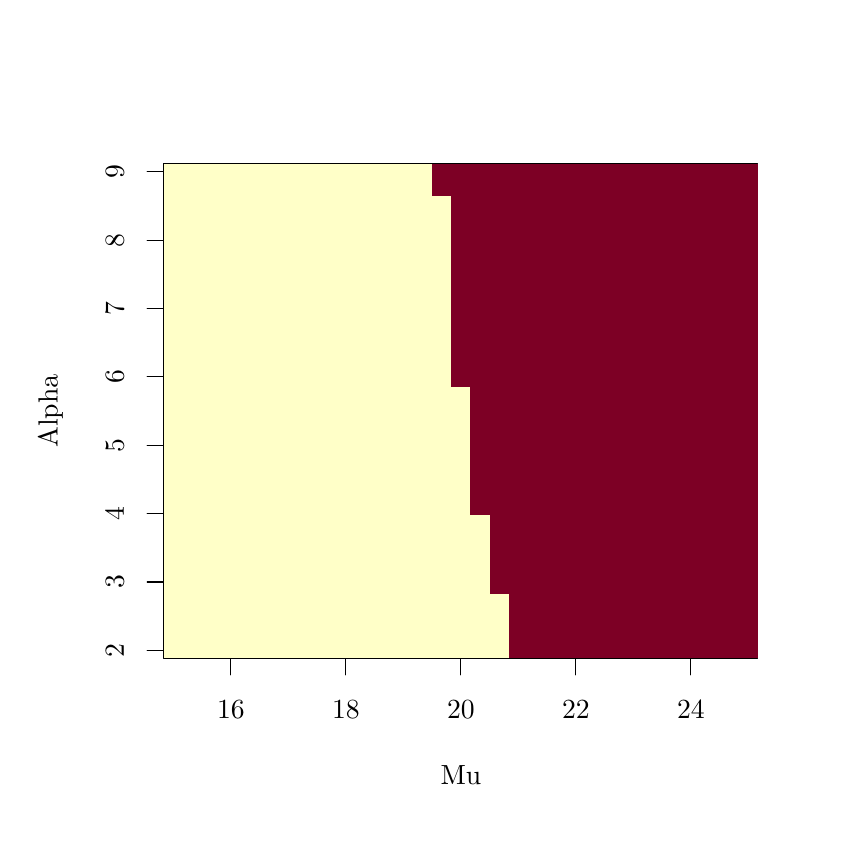
\begin{tikzpicture}[x=1pt,y=1pt]
\definecolor{fillColor}{RGB}{255,255,255}
\path[use as bounding box,fill=fillColor,fill opacity=0.00] (0,0) rectangle (289.08,289.08);
\begin{scope}
\path[clip] (  0.00,  0.00) rectangle (289.08,289.08);
\definecolor{drawColor}{RGB}{0,0,0}

\path[draw=drawColor,line width= 0.4pt,line join=round,line cap=round] ( 73.44, 61.20) -- (239.64, 61.20);

\path[draw=drawColor,line width= 0.4pt,line join=round,line cap=round] ( 73.44, 61.20) -- ( 73.44, 55.20);

\path[draw=drawColor,line width= 0.4pt,line join=round,line cap=round] (114.99, 61.20) -- (114.99, 55.20);

\path[draw=drawColor,line width= 0.4pt,line join=round,line cap=round] (156.54, 61.20) -- (156.54, 55.20);

\path[draw=drawColor,line width= 0.4pt,line join=round,line cap=round] (198.09, 61.20) -- (198.09, 55.20);

\path[draw=drawColor,line width= 0.4pt,line join=round,line cap=round] (239.64, 61.20) -- (239.64, 55.20);

\node[text=drawColor,anchor=base,inner sep=0pt, outer sep=0pt, scale=  1.00] at ( 73.44, 39.60) {16};

\node[text=drawColor,anchor=base,inner sep=0pt, outer sep=0pt, scale=  1.00] at (114.99, 39.60) {18};

\node[text=drawColor,anchor=base,inner sep=0pt, outer sep=0pt, scale=  1.00] at (156.54, 39.60) {20};

\node[text=drawColor,anchor=base,inner sep=0pt, outer sep=0pt, scale=  1.00] at (198.09, 39.60) {22};

\node[text=drawColor,anchor=base,inner sep=0pt, outer sep=0pt, scale=  1.00] at (239.64, 39.60) {24};

\path[draw=drawColor,line width= 0.4pt,line join=round,line cap=round] ( 49.20, 64.08) -- ( 49.20,237.00);

\path[draw=drawColor,line width= 0.4pt,line join=round,line cap=round] ( 49.20, 64.08) -- ( 43.20, 64.08);

\path[draw=drawColor,line width= 0.4pt,line join=round,line cap=round] ( 49.20, 88.78) -- ( 43.20, 88.78);

\path[draw=drawColor,line width= 0.4pt,line join=round,line cap=round] ( 49.20,113.49) -- ( 43.20,113.49);

\path[draw=drawColor,line width= 0.4pt,line join=round,line cap=round] ( 49.20,138.19) -- ( 43.20,138.19);

\path[draw=drawColor,line width= 0.4pt,line join=round,line cap=round] ( 49.20,162.89) -- ( 43.20,162.89);

\path[draw=drawColor,line width= 0.4pt,line join=round,line cap=round] ( 49.20,187.59) -- ( 43.20,187.59);

\path[draw=drawColor,line width= 0.4pt,line join=round,line cap=round] ( 49.20,212.30) -- ( 43.20,212.30);

\path[draw=drawColor,line width= 0.4pt,line join=round,line cap=round] ( 49.20,237.00) -- ( 43.20,237.00);

\node[text=drawColor,rotate= 90.00,anchor=base,inner sep=0pt, outer sep=0pt, scale=  1.00] at ( 34.80, 64.08) {2};

\node[text=drawColor,rotate= 90.00,anchor=base,inner sep=0pt, outer sep=0pt, scale=  1.00] at ( 34.80, 88.78) {3};

\node[text=drawColor,rotate= 90.00,anchor=base,inner sep=0pt, outer sep=0pt, scale=  1.00] at ( 34.80,113.49) {4};

\node[text=drawColor,rotate= 90.00,anchor=base,inner sep=0pt, outer sep=0pt, scale=  1.00] at ( 34.80,138.19) {5};

\node[text=drawColor,rotate= 90.00,anchor=base,inner sep=0pt, outer sep=0pt, scale=  1.00] at ( 34.80,162.89) {6};

\node[text=drawColor,rotate= 90.00,anchor=base,inner sep=0pt, outer sep=0pt, scale=  1.00] at ( 34.80,187.59) {7};

\node[text=drawColor,rotate= 90.00,anchor=base,inner sep=0pt, outer sep=0pt, scale=  1.00] at ( 34.80,212.30) {8};

\node[text=drawColor,rotate= 90.00,anchor=base,inner sep=0pt, outer sep=0pt, scale=  1.00] at ( 34.80,237.00) {9};

\path[draw=drawColor,line width= 0.4pt,line join=round,line cap=round] ( 49.20, 61.20) --
	(263.88, 61.20) --
	(263.88,239.88) --
	( 49.20,239.88) --
	( 49.20, 61.20);
\end{scope}
\begin{scope}
\path[clip] (  0.00,  0.00) rectangle (289.08,289.08);
\definecolor{drawColor}{RGB}{0,0,0}

\node[text=drawColor,anchor=base,inner sep=0pt, outer sep=0pt, scale=  1.00] at (156.54, 15.60) {Mu};

\node[text=drawColor,rotate= 90.00,anchor=base,inner sep=0pt, outer sep=0pt, scale=  1.00] at ( 10.80,150.54) {Alpha};
\end{scope}
\begin{scope}
\path[clip] ( 49.20, 61.20) rectangle (263.88,239.88);
\definecolor{fillColor}{RGB}{255,255,200}

\path[fill=fillColor] ( 49.20, 61.20) rectangle ( 56.13, 66.96);

\path[fill=fillColor] ( 49.20, 66.96) rectangle ( 56.13, 72.73);

\path[fill=fillColor] ( 49.20, 72.73) rectangle ( 56.13, 78.49);

\path[fill=fillColor] ( 49.20, 78.49) rectangle ( 56.13, 84.26);

\path[fill=fillColor] ( 49.20, 84.26) rectangle ( 56.13, 90.02);

\path[fill=fillColor] ( 49.20, 90.02) rectangle ( 56.13, 95.78);

\path[fill=fillColor] ( 49.20, 95.78) rectangle ( 56.13,101.55);

\path[fill=fillColor] ( 49.20,101.55) rectangle ( 56.13,107.31);

\path[fill=fillColor] ( 49.20,107.31) rectangle ( 56.13,113.07);

\path[fill=fillColor] ( 49.20,113.07) rectangle ( 56.13,118.84);

\path[fill=fillColor] ( 49.20,118.84) rectangle ( 56.13,124.60);

\path[fill=fillColor] ( 49.20,124.60) rectangle ( 56.13,130.37);

\path[fill=fillColor] ( 49.20,130.37) rectangle ( 56.13,136.13);

\path[fill=fillColor] ( 49.20,136.13) rectangle ( 56.13,141.89);

\path[fill=fillColor] ( 49.20,141.89) rectangle ( 56.13,147.66);

\path[fill=fillColor] ( 49.20,147.66) rectangle ( 56.13,153.42);

\path[fill=fillColor] ( 49.20,153.42) rectangle ( 56.13,159.19);

\path[fill=fillColor] ( 49.20,159.19) rectangle ( 56.13,164.95);

\path[fill=fillColor] ( 49.20,164.95) rectangle ( 56.13,170.71);

\path[fill=fillColor] ( 49.20,170.71) rectangle ( 56.13,176.48);

\path[fill=fillColor] ( 49.20,176.48) rectangle ( 56.13,182.24);

\path[fill=fillColor] ( 49.20,182.24) rectangle ( 56.13,188.01);

\path[fill=fillColor] ( 49.20,188.01) rectangle ( 56.13,193.77);

\path[fill=fillColor] ( 49.20,193.77) rectangle ( 56.13,199.53);

\path[fill=fillColor] ( 49.20,199.53) rectangle ( 56.13,205.30);

\path[fill=fillColor] ( 49.20,205.30) rectangle ( 56.13,211.06);

\path[fill=fillColor] ( 49.20,211.06) rectangle ( 56.13,216.82);

\path[fill=fillColor] ( 49.20,216.82) rectangle ( 56.13,222.59);

\path[fill=fillColor] ( 49.20,222.59) rectangle ( 56.13,228.35);

\path[fill=fillColor] ( 49.20,228.35) rectangle ( 56.13,234.12);

\path[fill=fillColor] ( 49.20,234.12) rectangle ( 56.13,239.88);

\path[fill=fillColor] ( 56.13, 61.20) rectangle ( 63.05, 66.96);

\path[fill=fillColor] ( 56.13, 66.96) rectangle ( 63.05, 72.73);

\path[fill=fillColor] ( 56.13, 72.73) rectangle ( 63.05, 78.49);

\path[fill=fillColor] ( 56.13, 78.49) rectangle ( 63.05, 84.26);

\path[fill=fillColor] ( 56.13, 84.26) rectangle ( 63.05, 90.02);

\path[fill=fillColor] ( 56.13, 90.02) rectangle ( 63.05, 95.78);

\path[fill=fillColor] ( 56.13, 95.78) rectangle ( 63.05,101.55);

\path[fill=fillColor] ( 56.13,101.55) rectangle ( 63.05,107.31);

\path[fill=fillColor] ( 56.13,107.31) rectangle ( 63.05,113.07);

\path[fill=fillColor] ( 56.13,113.07) rectangle ( 63.05,118.84);

\path[fill=fillColor] ( 56.13,118.84) rectangle ( 63.05,124.60);

\path[fill=fillColor] ( 56.13,124.60) rectangle ( 63.05,130.37);

\path[fill=fillColor] ( 56.13,130.37) rectangle ( 63.05,136.13);

\path[fill=fillColor] ( 56.13,136.13) rectangle ( 63.05,141.89);

\path[fill=fillColor] ( 56.13,141.89) rectangle ( 63.05,147.66);

\path[fill=fillColor] ( 56.13,147.66) rectangle ( 63.05,153.42);

\path[fill=fillColor] ( 56.13,153.42) rectangle ( 63.05,159.19);

\path[fill=fillColor] ( 56.13,159.19) rectangle ( 63.05,164.95);

\path[fill=fillColor] ( 56.13,164.95) rectangle ( 63.05,170.71);

\path[fill=fillColor] ( 56.13,170.71) rectangle ( 63.05,176.48);

\path[fill=fillColor] ( 56.13,176.48) rectangle ( 63.05,182.24);

\path[fill=fillColor] ( 56.13,182.24) rectangle ( 63.05,188.01);

\path[fill=fillColor] ( 56.13,188.01) rectangle ( 63.05,193.77);

\path[fill=fillColor] ( 56.13,193.77) rectangle ( 63.05,199.53);

\path[fill=fillColor] ( 56.13,199.53) rectangle ( 63.05,205.30);

\path[fill=fillColor] ( 56.13,205.30) rectangle ( 63.05,211.06);

\path[fill=fillColor] ( 56.13,211.06) rectangle ( 63.05,216.82);

\path[fill=fillColor] ( 56.13,216.82) rectangle ( 63.05,222.59);

\path[fill=fillColor] ( 56.13,222.59) rectangle ( 63.05,228.35);

\path[fill=fillColor] ( 56.13,228.35) rectangle ( 63.05,234.12);

\path[fill=fillColor] ( 56.13,234.12) rectangle ( 63.05,239.88);

\path[fill=fillColor] ( 63.05, 61.20) rectangle ( 69.98, 66.96);

\path[fill=fillColor] ( 63.05, 66.96) rectangle ( 69.98, 72.73);

\path[fill=fillColor] ( 63.05, 72.73) rectangle ( 69.98, 78.49);

\path[fill=fillColor] ( 63.05, 78.49) rectangle ( 69.98, 84.26);

\path[fill=fillColor] ( 63.05, 84.26) rectangle ( 69.98, 90.02);

\path[fill=fillColor] ( 63.05, 90.02) rectangle ( 69.98, 95.78);

\path[fill=fillColor] ( 63.05, 95.78) rectangle ( 69.98,101.55);

\path[fill=fillColor] ( 63.05,101.55) rectangle ( 69.98,107.31);

\path[fill=fillColor] ( 63.05,107.31) rectangle ( 69.98,113.07);

\path[fill=fillColor] ( 63.05,113.07) rectangle ( 69.98,118.84);

\path[fill=fillColor] ( 63.05,118.84) rectangle ( 69.98,124.60);

\path[fill=fillColor] ( 63.05,124.60) rectangle ( 69.98,130.37);

\path[fill=fillColor] ( 63.05,130.37) rectangle ( 69.98,136.13);

\path[fill=fillColor] ( 63.05,136.13) rectangle ( 69.98,141.89);

\path[fill=fillColor] ( 63.05,141.89) rectangle ( 69.98,147.66);

\path[fill=fillColor] ( 63.05,147.66) rectangle ( 69.98,153.42);

\path[fill=fillColor] ( 63.05,153.42) rectangle ( 69.98,159.19);

\path[fill=fillColor] ( 63.05,159.19) rectangle ( 69.98,164.95);

\path[fill=fillColor] ( 63.05,164.95) rectangle ( 69.98,170.71);

\path[fill=fillColor] ( 63.05,170.71) rectangle ( 69.98,176.48);

\path[fill=fillColor] ( 63.05,176.48) rectangle ( 69.98,182.24);

\path[fill=fillColor] ( 63.05,182.24) rectangle ( 69.98,188.01);

\path[fill=fillColor] ( 63.05,188.01) rectangle ( 69.98,193.77);

\path[fill=fillColor] ( 63.05,193.77) rectangle ( 69.98,199.53);

\path[fill=fillColor] ( 63.05,199.53) rectangle ( 69.98,205.30);

\path[fill=fillColor] ( 63.05,205.30) rectangle ( 69.98,211.06);

\path[fill=fillColor] ( 63.05,211.06) rectangle ( 69.98,216.82);

\path[fill=fillColor] ( 63.05,216.82) rectangle ( 69.98,222.59);

\path[fill=fillColor] ( 63.05,222.59) rectangle ( 69.98,228.35);

\path[fill=fillColor] ( 63.05,228.35) rectangle ( 69.98,234.12);

\path[fill=fillColor] ( 63.05,234.12) rectangle ( 69.98,239.88);

\path[fill=fillColor] ( 69.98, 61.20) rectangle ( 76.90, 66.96);

\path[fill=fillColor] ( 69.98, 66.96) rectangle ( 76.90, 72.73);

\path[fill=fillColor] ( 69.98, 72.73) rectangle ( 76.90, 78.49);

\path[fill=fillColor] ( 69.98, 78.49) rectangle ( 76.90, 84.26);

\path[fill=fillColor] ( 69.98, 84.26) rectangle ( 76.90, 90.02);

\path[fill=fillColor] ( 69.98, 90.02) rectangle ( 76.90, 95.78);

\path[fill=fillColor] ( 69.98, 95.78) rectangle ( 76.90,101.55);

\path[fill=fillColor] ( 69.98,101.55) rectangle ( 76.90,107.31);

\path[fill=fillColor] ( 69.98,107.31) rectangle ( 76.90,113.07);

\path[fill=fillColor] ( 69.98,113.07) rectangle ( 76.90,118.84);

\path[fill=fillColor] ( 69.98,118.84) rectangle ( 76.90,124.60);

\path[fill=fillColor] ( 69.98,124.60) rectangle ( 76.90,130.37);

\path[fill=fillColor] ( 69.98,130.37) rectangle ( 76.90,136.13);

\path[fill=fillColor] ( 69.98,136.13) rectangle ( 76.90,141.89);

\path[fill=fillColor] ( 69.98,141.89) rectangle ( 76.90,147.66);

\path[fill=fillColor] ( 69.98,147.66) rectangle ( 76.90,153.42);

\path[fill=fillColor] ( 69.98,153.42) rectangle ( 76.90,159.19);

\path[fill=fillColor] ( 69.98,159.19) rectangle ( 76.90,164.95);

\path[fill=fillColor] ( 69.98,164.95) rectangle ( 76.90,170.71);

\path[fill=fillColor] ( 69.98,170.71) rectangle ( 76.90,176.48);

\path[fill=fillColor] ( 69.98,176.48) rectangle ( 76.90,182.24);

\path[fill=fillColor] ( 69.98,182.24) rectangle ( 76.90,188.01);

\path[fill=fillColor] ( 69.98,188.01) rectangle ( 76.90,193.77);

\path[fill=fillColor] ( 69.98,193.77) rectangle ( 76.90,199.53);

\path[fill=fillColor] ( 69.98,199.53) rectangle ( 76.90,205.30);

\path[fill=fillColor] ( 69.98,205.30) rectangle ( 76.90,211.06);

\path[fill=fillColor] ( 69.98,211.06) rectangle ( 76.90,216.82);

\path[fill=fillColor] ( 69.98,216.82) rectangle ( 76.90,222.59);

\path[fill=fillColor] ( 69.98,222.59) rectangle ( 76.90,228.35);

\path[fill=fillColor] ( 69.98,228.35) rectangle ( 76.90,234.12);

\path[fill=fillColor] ( 69.98,234.12) rectangle ( 76.90,239.88);

\path[fill=fillColor] ( 76.90, 61.20) rectangle ( 83.83, 66.96);

\path[fill=fillColor] ( 76.90, 66.96) rectangle ( 83.83, 72.73);

\path[fill=fillColor] ( 76.90, 72.73) rectangle ( 83.83, 78.49);

\path[fill=fillColor] ( 76.90, 78.49) rectangle ( 83.83, 84.26);

\path[fill=fillColor] ( 76.90, 84.26) rectangle ( 83.83, 90.02);

\path[fill=fillColor] ( 76.90, 90.02) rectangle ( 83.83, 95.78);

\path[fill=fillColor] ( 76.90, 95.78) rectangle ( 83.83,101.55);

\path[fill=fillColor] ( 76.90,101.55) rectangle ( 83.83,107.31);

\path[fill=fillColor] ( 76.90,107.31) rectangle ( 83.83,113.07);

\path[fill=fillColor] ( 76.90,113.07) rectangle ( 83.83,118.84);

\path[fill=fillColor] ( 76.90,118.84) rectangle ( 83.83,124.60);

\path[fill=fillColor] ( 76.90,124.60) rectangle ( 83.83,130.37);

\path[fill=fillColor] ( 76.90,130.37) rectangle ( 83.83,136.13);

\path[fill=fillColor] ( 76.90,136.13) rectangle ( 83.83,141.89);

\path[fill=fillColor] ( 76.90,141.89) rectangle ( 83.83,147.66);

\path[fill=fillColor] ( 76.90,147.66) rectangle ( 83.83,153.42);

\path[fill=fillColor] ( 76.90,153.42) rectangle ( 83.83,159.19);

\path[fill=fillColor] ( 76.90,159.19) rectangle ( 83.83,164.95);

\path[fill=fillColor] ( 76.90,164.95) rectangle ( 83.83,170.71);

\path[fill=fillColor] ( 76.90,170.71) rectangle ( 83.83,176.48);

\path[fill=fillColor] ( 76.90,176.48) rectangle ( 83.83,182.24);

\path[fill=fillColor] ( 76.90,182.24) rectangle ( 83.83,188.01);

\path[fill=fillColor] ( 76.90,188.01) rectangle ( 83.83,193.77);

\path[fill=fillColor] ( 76.90,193.77) rectangle ( 83.83,199.53);

\path[fill=fillColor] ( 76.90,199.53) rectangle ( 83.83,205.30);

\path[fill=fillColor] ( 76.90,205.30) rectangle ( 83.83,211.06);

\path[fill=fillColor] ( 76.90,211.06) rectangle ( 83.83,216.82);

\path[fill=fillColor] ( 76.90,216.82) rectangle ( 83.83,222.59);

\path[fill=fillColor] ( 76.90,222.59) rectangle ( 83.83,228.35);

\path[fill=fillColor] ( 76.90,228.35) rectangle ( 83.83,234.12);

\path[fill=fillColor] ( 76.90,234.12) rectangle ( 83.83,239.88);

\path[fill=fillColor] ( 83.83, 61.20) rectangle ( 90.75, 66.96);

\path[fill=fillColor] ( 83.83, 66.96) rectangle ( 90.75, 72.73);

\path[fill=fillColor] ( 83.83, 72.73) rectangle ( 90.75, 78.49);

\path[fill=fillColor] ( 83.83, 78.49) rectangle ( 90.75, 84.26);

\path[fill=fillColor] ( 83.83, 84.26) rectangle ( 90.75, 90.02);

\path[fill=fillColor] ( 83.83, 90.02) rectangle ( 90.75, 95.78);

\path[fill=fillColor] ( 83.83, 95.78) rectangle ( 90.75,101.55);

\path[fill=fillColor] ( 83.83,101.55) rectangle ( 90.75,107.31);

\path[fill=fillColor] ( 83.83,107.31) rectangle ( 90.75,113.07);

\path[fill=fillColor] ( 83.83,113.07) rectangle ( 90.75,118.84);

\path[fill=fillColor] ( 83.83,118.84) rectangle ( 90.75,124.60);

\path[fill=fillColor] ( 83.83,124.60) rectangle ( 90.75,130.37);

\path[fill=fillColor] ( 83.83,130.37) rectangle ( 90.75,136.13);

\path[fill=fillColor] ( 83.83,136.13) rectangle ( 90.75,141.89);

\path[fill=fillColor] ( 83.83,141.89) rectangle ( 90.75,147.66);

\path[fill=fillColor] ( 83.83,147.66) rectangle ( 90.75,153.42);

\path[fill=fillColor] ( 83.83,153.42) rectangle ( 90.75,159.19);

\path[fill=fillColor] ( 83.83,159.19) rectangle ( 90.75,164.95);

\path[fill=fillColor] ( 83.83,164.95) rectangle ( 90.75,170.71);

\path[fill=fillColor] ( 83.83,170.71) rectangle ( 90.75,176.48);

\path[fill=fillColor] ( 83.83,176.48) rectangle ( 90.75,182.24);

\path[fill=fillColor] ( 83.83,182.24) rectangle ( 90.75,188.01);

\path[fill=fillColor] ( 83.83,188.01) rectangle ( 90.75,193.77);

\path[fill=fillColor] ( 83.83,193.77) rectangle ( 90.75,199.53);

\path[fill=fillColor] ( 83.83,199.53) rectangle ( 90.75,205.30);

\path[fill=fillColor] ( 83.83,205.30) rectangle ( 90.75,211.06);

\path[fill=fillColor] ( 83.83,211.06) rectangle ( 90.75,216.82);

\path[fill=fillColor] ( 83.83,216.82) rectangle ( 90.75,222.59);

\path[fill=fillColor] ( 83.83,222.59) rectangle ( 90.75,228.35);

\path[fill=fillColor] ( 83.83,228.35) rectangle ( 90.75,234.12);

\path[fill=fillColor] ( 83.83,234.12) rectangle ( 90.75,239.88);

\path[fill=fillColor] ( 90.75, 61.20) rectangle ( 97.68, 66.96);

\path[fill=fillColor] ( 90.75, 66.96) rectangle ( 97.68, 72.73);

\path[fill=fillColor] ( 90.75, 72.73) rectangle ( 97.68, 78.49);

\path[fill=fillColor] ( 90.75, 78.49) rectangle ( 97.68, 84.26);

\path[fill=fillColor] ( 90.75, 84.26) rectangle ( 97.68, 90.02);

\path[fill=fillColor] ( 90.75, 90.02) rectangle ( 97.68, 95.78);

\path[fill=fillColor] ( 90.75, 95.78) rectangle ( 97.68,101.55);

\path[fill=fillColor] ( 90.75,101.55) rectangle ( 97.68,107.31);

\path[fill=fillColor] ( 90.75,107.31) rectangle ( 97.68,113.07);

\path[fill=fillColor] ( 90.75,113.07) rectangle ( 97.68,118.84);

\path[fill=fillColor] ( 90.75,118.84) rectangle ( 97.68,124.60);

\path[fill=fillColor] ( 90.75,124.60) rectangle ( 97.68,130.37);

\path[fill=fillColor] ( 90.75,130.37) rectangle ( 97.68,136.13);

\path[fill=fillColor] ( 90.75,136.13) rectangle ( 97.68,141.89);

\path[fill=fillColor] ( 90.75,141.89) rectangle ( 97.68,147.66);

\path[fill=fillColor] ( 90.75,147.66) rectangle ( 97.68,153.42);

\path[fill=fillColor] ( 90.75,153.42) rectangle ( 97.68,159.19);

\path[fill=fillColor] ( 90.75,159.19) rectangle ( 97.68,164.95);

\path[fill=fillColor] ( 90.75,164.95) rectangle ( 97.68,170.71);

\path[fill=fillColor] ( 90.75,170.71) rectangle ( 97.68,176.48);

\path[fill=fillColor] ( 90.75,176.48) rectangle ( 97.68,182.24);

\path[fill=fillColor] ( 90.75,182.24) rectangle ( 97.68,188.01);

\path[fill=fillColor] ( 90.75,188.01) rectangle ( 97.68,193.77);

\path[fill=fillColor] ( 90.75,193.77) rectangle ( 97.68,199.53);

\path[fill=fillColor] ( 90.75,199.53) rectangle ( 97.68,205.30);

\path[fill=fillColor] ( 90.75,205.30) rectangle ( 97.68,211.06);

\path[fill=fillColor] ( 90.75,211.06) rectangle ( 97.68,216.82);

\path[fill=fillColor] ( 90.75,216.82) rectangle ( 97.68,222.59);

\path[fill=fillColor] ( 90.75,222.59) rectangle ( 97.68,228.35);

\path[fill=fillColor] ( 90.75,228.35) rectangle ( 97.68,234.12);

\path[fill=fillColor] ( 90.75,234.12) rectangle ( 97.68,239.88);

\path[fill=fillColor] ( 97.68, 61.20) rectangle (104.60, 66.96);

\path[fill=fillColor] ( 97.68, 66.96) rectangle (104.60, 72.73);

\path[fill=fillColor] ( 97.68, 72.73) rectangle (104.60, 78.49);

\path[fill=fillColor] ( 97.68, 78.49) rectangle (104.60, 84.26);

\path[fill=fillColor] ( 97.68, 84.26) rectangle (104.60, 90.02);

\path[fill=fillColor] ( 97.68, 90.02) rectangle (104.60, 95.78);

\path[fill=fillColor] ( 97.68, 95.78) rectangle (104.60,101.55);

\path[fill=fillColor] ( 97.68,101.55) rectangle (104.60,107.31);

\path[fill=fillColor] ( 97.68,107.31) rectangle (104.60,113.07);

\path[fill=fillColor] ( 97.68,113.07) rectangle (104.60,118.84);

\path[fill=fillColor] ( 97.68,118.84) rectangle (104.60,124.60);

\path[fill=fillColor] ( 97.68,124.60) rectangle (104.60,130.37);

\path[fill=fillColor] ( 97.68,130.37) rectangle (104.60,136.13);

\path[fill=fillColor] ( 97.68,136.13) rectangle (104.60,141.89);

\path[fill=fillColor] ( 97.68,141.89) rectangle (104.60,147.66);

\path[fill=fillColor] ( 97.68,147.66) rectangle (104.60,153.42);

\path[fill=fillColor] ( 97.68,153.42) rectangle (104.60,159.19);

\path[fill=fillColor] ( 97.68,159.19) rectangle (104.60,164.95);

\path[fill=fillColor] ( 97.68,164.95) rectangle (104.60,170.71);

\path[fill=fillColor] ( 97.68,170.71) rectangle (104.60,176.48);

\path[fill=fillColor] ( 97.68,176.48) rectangle (104.60,182.24);

\path[fill=fillColor] ( 97.68,182.24) rectangle (104.60,188.01);

\path[fill=fillColor] ( 97.68,188.01) rectangle (104.60,193.77);

\path[fill=fillColor] ( 97.68,193.77) rectangle (104.60,199.53);

\path[fill=fillColor] ( 97.68,199.53) rectangle (104.60,205.30);

\path[fill=fillColor] ( 97.68,205.30) rectangle (104.60,211.06);

\path[fill=fillColor] ( 97.68,211.06) rectangle (104.60,216.82);

\path[fill=fillColor] ( 97.68,216.82) rectangle (104.60,222.59);

\path[fill=fillColor] ( 97.68,222.59) rectangle (104.60,228.35);

\path[fill=fillColor] ( 97.68,228.35) rectangle (104.60,234.12);

\path[fill=fillColor] ( 97.68,234.12) rectangle (104.60,239.88);

\path[fill=fillColor] (104.60, 61.20) rectangle (111.53, 66.96);

\path[fill=fillColor] (104.60, 66.96) rectangle (111.53, 72.73);

\path[fill=fillColor] (104.60, 72.73) rectangle (111.53, 78.49);

\path[fill=fillColor] (104.60, 78.49) rectangle (111.53, 84.26);

\path[fill=fillColor] (104.60, 84.26) rectangle (111.53, 90.02);

\path[fill=fillColor] (104.60, 90.02) rectangle (111.53, 95.78);

\path[fill=fillColor] (104.60, 95.78) rectangle (111.53,101.55);

\path[fill=fillColor] (104.60,101.55) rectangle (111.53,107.31);

\path[fill=fillColor] (104.60,107.31) rectangle (111.53,113.07);

\path[fill=fillColor] (104.60,113.07) rectangle (111.53,118.84);

\path[fill=fillColor] (104.60,118.84) rectangle (111.53,124.60);

\path[fill=fillColor] (104.60,124.60) rectangle (111.53,130.37);

\path[fill=fillColor] (104.60,130.37) rectangle (111.53,136.13);

\path[fill=fillColor] (104.60,136.13) rectangle (111.53,141.89);

\path[fill=fillColor] (104.60,141.89) rectangle (111.53,147.66);

\path[fill=fillColor] (104.60,147.66) rectangle (111.53,153.42);

\path[fill=fillColor] (104.60,153.42) rectangle (111.53,159.19);

\path[fill=fillColor] (104.60,159.19) rectangle (111.53,164.95);

\path[fill=fillColor] (104.60,164.95) rectangle (111.53,170.71);

\path[fill=fillColor] (104.60,170.71) rectangle (111.53,176.48);

\path[fill=fillColor] (104.60,176.48) rectangle (111.53,182.24);

\path[fill=fillColor] (104.60,182.24) rectangle (111.53,188.01);

\path[fill=fillColor] (104.60,188.01) rectangle (111.53,193.77);

\path[fill=fillColor] (104.60,193.77) rectangle (111.53,199.53);

\path[fill=fillColor] (104.60,199.53) rectangle (111.53,205.30);

\path[fill=fillColor] (104.60,205.30) rectangle (111.53,211.06);

\path[fill=fillColor] (104.60,211.06) rectangle (111.53,216.82);

\path[fill=fillColor] (104.60,216.82) rectangle (111.53,222.59);

\path[fill=fillColor] (104.60,222.59) rectangle (111.53,228.35);

\path[fill=fillColor] (104.60,228.35) rectangle (111.53,234.12);

\path[fill=fillColor] (104.60,234.12) rectangle (111.53,239.88);

\path[fill=fillColor] (111.53, 61.20) rectangle (118.45, 66.96);

\path[fill=fillColor] (111.53, 66.96) rectangle (118.45, 72.73);

\path[fill=fillColor] (111.53, 72.73) rectangle (118.45, 78.49);

\path[fill=fillColor] (111.53, 78.49) rectangle (118.45, 84.26);

\path[fill=fillColor] (111.53, 84.26) rectangle (118.45, 90.02);

\path[fill=fillColor] (111.53, 90.02) rectangle (118.45, 95.78);

\path[fill=fillColor] (111.53, 95.78) rectangle (118.45,101.55);

\path[fill=fillColor] (111.53,101.55) rectangle (118.45,107.31);

\path[fill=fillColor] (111.53,107.31) rectangle (118.45,113.07);

\path[fill=fillColor] (111.53,113.07) rectangle (118.45,118.84);

\path[fill=fillColor] (111.53,118.84) rectangle (118.45,124.60);

\path[fill=fillColor] (111.53,124.60) rectangle (118.45,130.37);

\path[fill=fillColor] (111.53,130.37) rectangle (118.45,136.13);

\path[fill=fillColor] (111.53,136.13) rectangle (118.45,141.89);

\path[fill=fillColor] (111.53,141.89) rectangle (118.45,147.66);

\path[fill=fillColor] (111.53,147.66) rectangle (118.45,153.42);

\path[fill=fillColor] (111.53,153.42) rectangle (118.45,159.19);

\path[fill=fillColor] (111.53,159.19) rectangle (118.45,164.95);

\path[fill=fillColor] (111.53,164.95) rectangle (118.45,170.71);

\path[fill=fillColor] (111.53,170.71) rectangle (118.45,176.48);

\path[fill=fillColor] (111.53,176.48) rectangle (118.45,182.24);

\path[fill=fillColor] (111.53,182.24) rectangle (118.45,188.01);

\path[fill=fillColor] (111.53,188.01) rectangle (118.45,193.77);

\path[fill=fillColor] (111.53,193.77) rectangle (118.45,199.53);

\path[fill=fillColor] (111.53,199.53) rectangle (118.45,205.30);

\path[fill=fillColor] (111.53,205.30) rectangle (118.45,211.06);

\path[fill=fillColor] (111.53,211.06) rectangle (118.45,216.82);

\path[fill=fillColor] (111.53,216.82) rectangle (118.45,222.59);

\path[fill=fillColor] (111.53,222.59) rectangle (118.45,228.35);

\path[fill=fillColor] (111.53,228.35) rectangle (118.45,234.12);

\path[fill=fillColor] (111.53,234.12) rectangle (118.45,239.88);

\path[fill=fillColor] (118.45, 61.20) rectangle (125.38, 66.96);

\path[fill=fillColor] (118.45, 66.96) rectangle (125.38, 72.73);

\path[fill=fillColor] (118.45, 72.73) rectangle (125.38, 78.49);

\path[fill=fillColor] (118.45, 78.49) rectangle (125.38, 84.26);

\path[fill=fillColor] (118.45, 84.26) rectangle (125.38, 90.02);

\path[fill=fillColor] (118.45, 90.02) rectangle (125.38, 95.78);

\path[fill=fillColor] (118.45, 95.78) rectangle (125.38,101.55);

\path[fill=fillColor] (118.45,101.55) rectangle (125.38,107.31);

\path[fill=fillColor] (118.45,107.31) rectangle (125.38,113.07);

\path[fill=fillColor] (118.45,113.07) rectangle (125.38,118.84);

\path[fill=fillColor] (118.45,118.84) rectangle (125.38,124.60);

\path[fill=fillColor] (118.45,124.60) rectangle (125.38,130.37);

\path[fill=fillColor] (118.45,130.37) rectangle (125.38,136.13);

\path[fill=fillColor] (118.45,136.13) rectangle (125.38,141.89);

\path[fill=fillColor] (118.45,141.89) rectangle (125.38,147.66);

\path[fill=fillColor] (118.45,147.66) rectangle (125.38,153.42);

\path[fill=fillColor] (118.45,153.42) rectangle (125.38,159.19);

\path[fill=fillColor] (118.45,159.19) rectangle (125.38,164.95);

\path[fill=fillColor] (118.45,164.95) rectangle (125.38,170.71);

\path[fill=fillColor] (118.45,170.71) rectangle (125.38,176.48);

\path[fill=fillColor] (118.45,176.48) rectangle (125.38,182.24);

\path[fill=fillColor] (118.45,182.24) rectangle (125.38,188.01);

\path[fill=fillColor] (118.45,188.01) rectangle (125.38,193.77);

\path[fill=fillColor] (118.45,193.77) rectangle (125.38,199.53);

\path[fill=fillColor] (118.45,199.53) rectangle (125.38,205.30);

\path[fill=fillColor] (118.45,205.30) rectangle (125.38,211.06);

\path[fill=fillColor] (118.45,211.06) rectangle (125.38,216.82);

\path[fill=fillColor] (118.45,216.82) rectangle (125.38,222.59);

\path[fill=fillColor] (118.45,222.59) rectangle (125.38,228.35);

\path[fill=fillColor] (118.45,228.35) rectangle (125.38,234.12);

\path[fill=fillColor] (118.45,234.12) rectangle (125.38,239.88);

\path[fill=fillColor] (125.38, 61.20) rectangle (132.30, 66.96);

\path[fill=fillColor] (125.38, 66.96) rectangle (132.30, 72.73);

\path[fill=fillColor] (125.38, 72.73) rectangle (132.30, 78.49);

\path[fill=fillColor] (125.38, 78.49) rectangle (132.30, 84.26);

\path[fill=fillColor] (125.38, 84.26) rectangle (132.30, 90.02);

\path[fill=fillColor] (125.38, 90.02) rectangle (132.30, 95.78);

\path[fill=fillColor] (125.38, 95.78) rectangle (132.30,101.55);

\path[fill=fillColor] (125.38,101.55) rectangle (132.30,107.31);

\path[fill=fillColor] (125.38,107.31) rectangle (132.30,113.07);

\path[fill=fillColor] (125.38,113.07) rectangle (132.30,118.84);

\path[fill=fillColor] (125.38,118.84) rectangle (132.30,124.60);

\path[fill=fillColor] (125.38,124.60) rectangle (132.30,130.37);

\path[fill=fillColor] (125.38,130.37) rectangle (132.30,136.13);

\path[fill=fillColor] (125.38,136.13) rectangle (132.30,141.89);

\path[fill=fillColor] (125.38,141.89) rectangle (132.30,147.66);

\path[fill=fillColor] (125.38,147.66) rectangle (132.30,153.42);

\path[fill=fillColor] (125.38,153.42) rectangle (132.30,159.19);

\path[fill=fillColor] (125.38,159.19) rectangle (132.30,164.95);

\path[fill=fillColor] (125.38,164.95) rectangle (132.30,170.71);

\path[fill=fillColor] (125.38,170.71) rectangle (132.30,176.48);

\path[fill=fillColor] (125.38,176.48) rectangle (132.30,182.24);

\path[fill=fillColor] (125.38,182.24) rectangle (132.30,188.01);

\path[fill=fillColor] (125.38,188.01) rectangle (132.30,193.77);

\path[fill=fillColor] (125.38,193.77) rectangle (132.30,199.53);

\path[fill=fillColor] (125.38,199.53) rectangle (132.30,205.30);

\path[fill=fillColor] (125.38,205.30) rectangle (132.30,211.06);

\path[fill=fillColor] (125.38,211.06) rectangle (132.30,216.82);

\path[fill=fillColor] (125.38,216.82) rectangle (132.30,222.59);

\path[fill=fillColor] (125.38,222.59) rectangle (132.30,228.35);

\path[fill=fillColor] (125.38,228.35) rectangle (132.30,234.12);

\path[fill=fillColor] (125.38,234.12) rectangle (132.30,239.88);

\path[fill=fillColor] (132.30, 61.20) rectangle (139.23, 66.96);

\path[fill=fillColor] (132.30, 66.96) rectangle (139.23, 72.73);

\path[fill=fillColor] (132.30, 72.73) rectangle (139.23, 78.49);

\path[fill=fillColor] (132.30, 78.49) rectangle (139.23, 84.26);

\path[fill=fillColor] (132.30, 84.26) rectangle (139.23, 90.02);

\path[fill=fillColor] (132.30, 90.02) rectangle (139.23, 95.78);

\path[fill=fillColor] (132.30, 95.78) rectangle (139.23,101.55);

\path[fill=fillColor] (132.30,101.55) rectangle (139.23,107.31);

\path[fill=fillColor] (132.30,107.31) rectangle (139.23,113.07);

\path[fill=fillColor] (132.30,113.07) rectangle (139.23,118.84);

\path[fill=fillColor] (132.30,118.84) rectangle (139.23,124.60);

\path[fill=fillColor] (132.30,124.60) rectangle (139.23,130.37);

\path[fill=fillColor] (132.30,130.37) rectangle (139.23,136.13);

\path[fill=fillColor] (132.30,136.13) rectangle (139.23,141.89);

\path[fill=fillColor] (132.30,141.89) rectangle (139.23,147.66);

\path[fill=fillColor] (132.30,147.66) rectangle (139.23,153.42);

\path[fill=fillColor] (132.30,153.42) rectangle (139.23,159.19);

\path[fill=fillColor] (132.30,159.19) rectangle (139.23,164.95);

\path[fill=fillColor] (132.30,164.95) rectangle (139.23,170.71);

\path[fill=fillColor] (132.30,170.71) rectangle (139.23,176.48);

\path[fill=fillColor] (132.30,176.48) rectangle (139.23,182.24);

\path[fill=fillColor] (132.30,182.24) rectangle (139.23,188.01);

\path[fill=fillColor] (132.30,188.01) rectangle (139.23,193.77);

\path[fill=fillColor] (132.30,193.77) rectangle (139.23,199.53);

\path[fill=fillColor] (132.30,199.53) rectangle (139.23,205.30);

\path[fill=fillColor] (132.30,205.30) rectangle (139.23,211.06);

\path[fill=fillColor] (132.30,211.06) rectangle (139.23,216.82);

\path[fill=fillColor] (132.30,216.82) rectangle (139.23,222.59);

\path[fill=fillColor] (132.30,222.59) rectangle (139.23,228.35);

\path[fill=fillColor] (132.30,228.35) rectangle (139.23,234.12);

\path[fill=fillColor] (132.30,234.12) rectangle (139.23,239.88);

\path[fill=fillColor] (139.23, 61.20) rectangle (146.15, 66.96);

\path[fill=fillColor] (139.23, 66.96) rectangle (146.15, 72.73);

\path[fill=fillColor] (139.23, 72.73) rectangle (146.15, 78.49);

\path[fill=fillColor] (139.23, 78.49) rectangle (146.15, 84.26);

\path[fill=fillColor] (139.23, 84.26) rectangle (146.15, 90.02);

\path[fill=fillColor] (139.23, 90.02) rectangle (146.15, 95.78);

\path[fill=fillColor] (139.23, 95.78) rectangle (146.15,101.55);

\path[fill=fillColor] (139.23,101.55) rectangle (146.15,107.31);

\path[fill=fillColor] (139.23,107.31) rectangle (146.15,113.07);

\path[fill=fillColor] (139.23,113.07) rectangle (146.15,118.84);

\path[fill=fillColor] (139.23,118.84) rectangle (146.15,124.60);

\path[fill=fillColor] (139.23,124.60) rectangle (146.15,130.37);

\path[fill=fillColor] (139.23,130.37) rectangle (146.15,136.13);

\path[fill=fillColor] (139.23,136.13) rectangle (146.15,141.89);

\path[fill=fillColor] (139.23,141.89) rectangle (146.15,147.66);

\path[fill=fillColor] (139.23,147.66) rectangle (146.15,153.42);

\path[fill=fillColor] (139.23,153.42) rectangle (146.15,159.19);

\path[fill=fillColor] (139.23,159.19) rectangle (146.15,164.95);

\path[fill=fillColor] (139.23,164.95) rectangle (146.15,170.71);

\path[fill=fillColor] (139.23,170.71) rectangle (146.15,176.48);

\path[fill=fillColor] (139.23,176.48) rectangle (146.15,182.24);

\path[fill=fillColor] (139.23,182.24) rectangle (146.15,188.01);

\path[fill=fillColor] (139.23,188.01) rectangle (146.15,193.77);

\path[fill=fillColor] (139.23,193.77) rectangle (146.15,199.53);

\path[fill=fillColor] (139.23,199.53) rectangle (146.15,205.30);

\path[fill=fillColor] (139.23,205.30) rectangle (146.15,211.06);

\path[fill=fillColor] (139.23,211.06) rectangle (146.15,216.82);

\path[fill=fillColor] (139.23,216.82) rectangle (146.15,222.59);

\path[fill=fillColor] (139.23,222.59) rectangle (146.15,228.35);

\path[fill=fillColor] (139.23,228.35) rectangle (146.15,234.12);

\path[fill=fillColor] (139.23,234.12) rectangle (146.15,239.88);

\path[fill=fillColor] (146.15, 61.20) rectangle (153.08, 66.96);

\path[fill=fillColor] (146.15, 66.96) rectangle (153.08, 72.73);

\path[fill=fillColor] (146.15, 72.73) rectangle (153.08, 78.49);

\path[fill=fillColor] (146.15, 78.49) rectangle (153.08, 84.26);

\path[fill=fillColor] (146.15, 84.26) rectangle (153.08, 90.02);

\path[fill=fillColor] (146.15, 90.02) rectangle (153.08, 95.78);

\path[fill=fillColor] (146.15, 95.78) rectangle (153.08,101.55);

\path[fill=fillColor] (146.15,101.55) rectangle (153.08,107.31);

\path[fill=fillColor] (146.15,107.31) rectangle (153.08,113.07);

\path[fill=fillColor] (146.15,113.07) rectangle (153.08,118.84);

\path[fill=fillColor] (146.15,118.84) rectangle (153.08,124.60);

\path[fill=fillColor] (146.15,124.60) rectangle (153.08,130.37);

\path[fill=fillColor] (146.15,130.37) rectangle (153.08,136.13);

\path[fill=fillColor] (146.15,136.13) rectangle (153.08,141.89);

\path[fill=fillColor] (146.15,141.89) rectangle (153.08,147.66);

\path[fill=fillColor] (146.15,147.66) rectangle (153.08,153.42);

\path[fill=fillColor] (146.15,153.42) rectangle (153.08,159.19);

\path[fill=fillColor] (146.15,159.19) rectangle (153.08,164.95);

\path[fill=fillColor] (146.15,164.95) rectangle (153.08,170.71);

\path[fill=fillColor] (146.15,170.71) rectangle (153.08,176.48);

\path[fill=fillColor] (146.15,176.48) rectangle (153.08,182.24);

\path[fill=fillColor] (146.15,182.24) rectangle (153.08,188.01);

\path[fill=fillColor] (146.15,188.01) rectangle (153.08,193.77);

\path[fill=fillColor] (146.15,193.77) rectangle (153.08,199.53);

\path[fill=fillColor] (146.15,199.53) rectangle (153.08,205.30);

\path[fill=fillColor] (146.15,205.30) rectangle (153.08,211.06);

\path[fill=fillColor] (146.15,211.06) rectangle (153.08,216.82);

\path[fill=fillColor] (146.15,216.82) rectangle (153.08,222.59);

\path[fill=fillColor] (146.15,222.59) rectangle (153.08,228.35);
\definecolor{fillColor}{RGB}{125,0,37}

\path[fill=fillColor] (146.15,228.35) rectangle (153.08,234.12);

\path[fill=fillColor] (146.15,234.12) rectangle (153.08,239.88);
\definecolor{fillColor}{RGB}{255,255,200}

\path[fill=fillColor] (153.08, 61.20) rectangle (160.00, 66.96);

\path[fill=fillColor] (153.08, 66.96) rectangle (160.00, 72.73);

\path[fill=fillColor] (153.08, 72.73) rectangle (160.00, 78.49);

\path[fill=fillColor] (153.08, 78.49) rectangle (160.00, 84.26);

\path[fill=fillColor] (153.08, 84.26) rectangle (160.00, 90.02);

\path[fill=fillColor] (153.08, 90.02) rectangle (160.00, 95.78);

\path[fill=fillColor] (153.08, 95.78) rectangle (160.00,101.55);

\path[fill=fillColor] (153.08,101.55) rectangle (160.00,107.31);

\path[fill=fillColor] (153.08,107.31) rectangle (160.00,113.07);

\path[fill=fillColor] (153.08,113.07) rectangle (160.00,118.84);

\path[fill=fillColor] (153.08,118.84) rectangle (160.00,124.60);

\path[fill=fillColor] (153.08,124.60) rectangle (160.00,130.37);

\path[fill=fillColor] (153.08,130.37) rectangle (160.00,136.13);

\path[fill=fillColor] (153.08,136.13) rectangle (160.00,141.89);

\path[fill=fillColor] (153.08,141.89) rectangle (160.00,147.66);

\path[fill=fillColor] (153.08,147.66) rectangle (160.00,153.42);

\path[fill=fillColor] (153.08,153.42) rectangle (160.00,159.19);
\definecolor{fillColor}{RGB}{125,0,37}

\path[fill=fillColor] (153.08,159.19) rectangle (160.00,164.95);

\path[fill=fillColor] (153.08,164.95) rectangle (160.00,170.71);

\path[fill=fillColor] (153.08,170.71) rectangle (160.00,176.48);

\path[fill=fillColor] (153.08,176.48) rectangle (160.00,182.24);

\path[fill=fillColor] (153.08,182.24) rectangle (160.00,188.01);

\path[fill=fillColor] (153.08,188.01) rectangle (160.00,193.77);

\path[fill=fillColor] (153.08,193.77) rectangle (160.00,199.53);

\path[fill=fillColor] (153.08,199.53) rectangle (160.00,205.30);

\path[fill=fillColor] (153.08,205.30) rectangle (160.00,211.06);

\path[fill=fillColor] (153.08,211.06) rectangle (160.00,216.82);

\path[fill=fillColor] (153.08,216.82) rectangle (160.00,222.59);

\path[fill=fillColor] (153.08,222.59) rectangle (160.00,228.35);

\path[fill=fillColor] (153.08,228.35) rectangle (160.00,234.12);

\path[fill=fillColor] (153.08,234.12) rectangle (160.00,239.88);
\definecolor{fillColor}{RGB}{255,255,200}

\path[fill=fillColor] (160.00, 61.20) rectangle (166.93, 66.96);

\path[fill=fillColor] (160.00, 66.96) rectangle (166.93, 72.73);

\path[fill=fillColor] (160.00, 72.73) rectangle (166.93, 78.49);

\path[fill=fillColor] (160.00, 78.49) rectangle (166.93, 84.26);

\path[fill=fillColor] (160.00, 84.26) rectangle (166.93, 90.02);

\path[fill=fillColor] (160.00, 90.02) rectangle (166.93, 95.78);

\path[fill=fillColor] (160.00, 95.78) rectangle (166.93,101.55);

\path[fill=fillColor] (160.00,101.55) rectangle (166.93,107.31);

\path[fill=fillColor] (160.00,107.31) rectangle (166.93,113.07);
\definecolor{fillColor}{RGB}{125,0,37}

\path[fill=fillColor] (160.00,113.07) rectangle (166.93,118.84);

\path[fill=fillColor] (160.00,118.84) rectangle (166.93,124.60);

\path[fill=fillColor] (160.00,124.60) rectangle (166.93,130.37);

\path[fill=fillColor] (160.00,130.37) rectangle (166.93,136.13);

\path[fill=fillColor] (160.00,136.13) rectangle (166.93,141.89);

\path[fill=fillColor] (160.00,141.89) rectangle (166.93,147.66);

\path[fill=fillColor] (160.00,147.66) rectangle (166.93,153.42);

\path[fill=fillColor] (160.00,153.42) rectangle (166.93,159.19);

\path[fill=fillColor] (160.00,159.19) rectangle (166.93,164.95);

\path[fill=fillColor] (160.00,164.95) rectangle (166.93,170.71);

\path[fill=fillColor] (160.00,170.71) rectangle (166.93,176.48);

\path[fill=fillColor] (160.00,176.48) rectangle (166.93,182.24);

\path[fill=fillColor] (160.00,182.24) rectangle (166.93,188.01);

\path[fill=fillColor] (160.00,188.01) rectangle (166.93,193.77);

\path[fill=fillColor] (160.00,193.77) rectangle (166.93,199.53);

\path[fill=fillColor] (160.00,199.53) rectangle (166.93,205.30);

\path[fill=fillColor] (160.00,205.30) rectangle (166.93,211.06);

\path[fill=fillColor] (160.00,211.06) rectangle (166.93,216.82);

\path[fill=fillColor] (160.00,216.82) rectangle (166.93,222.59);

\path[fill=fillColor] (160.00,222.59) rectangle (166.93,228.35);

\path[fill=fillColor] (160.00,228.35) rectangle (166.93,234.12);

\path[fill=fillColor] (160.00,234.12) rectangle (166.93,239.88);
\definecolor{fillColor}{RGB}{255,255,200}

\path[fill=fillColor] (166.93, 61.20) rectangle (173.85, 66.96);

\path[fill=fillColor] (166.93, 66.96) rectangle (173.85, 72.73);

\path[fill=fillColor] (166.93, 72.73) rectangle (173.85, 78.49);

\path[fill=fillColor] (166.93, 78.49) rectangle (173.85, 84.26);
\definecolor{fillColor}{RGB}{125,0,37}

\path[fill=fillColor] (166.93, 84.26) rectangle (173.85, 90.02);

\path[fill=fillColor] (166.93, 90.02) rectangle (173.85, 95.78);

\path[fill=fillColor] (166.93, 95.78) rectangle (173.85,101.55);

\path[fill=fillColor] (166.93,101.55) rectangle (173.85,107.31);

\path[fill=fillColor] (166.93,107.31) rectangle (173.85,113.07);

\path[fill=fillColor] (166.93,113.07) rectangle (173.85,118.84);

\path[fill=fillColor] (166.93,118.84) rectangle (173.85,124.60);

\path[fill=fillColor] (166.93,124.60) rectangle (173.85,130.37);

\path[fill=fillColor] (166.93,130.37) rectangle (173.85,136.13);

\path[fill=fillColor] (166.93,136.13) rectangle (173.85,141.89);

\path[fill=fillColor] (166.93,141.89) rectangle (173.85,147.66);

\path[fill=fillColor] (166.93,147.66) rectangle (173.85,153.42);

\path[fill=fillColor] (166.93,153.42) rectangle (173.85,159.19);

\path[fill=fillColor] (166.93,159.19) rectangle (173.85,164.95);

\path[fill=fillColor] (166.93,164.95) rectangle (173.85,170.71);

\path[fill=fillColor] (166.93,170.71) rectangle (173.85,176.48);

\path[fill=fillColor] (166.93,176.48) rectangle (173.85,182.24);

\path[fill=fillColor] (166.93,182.24) rectangle (173.85,188.01);

\path[fill=fillColor] (166.93,188.01) rectangle (173.85,193.77);

\path[fill=fillColor] (166.93,193.77) rectangle (173.85,199.53);

\path[fill=fillColor] (166.93,199.53) rectangle (173.85,205.30);

\path[fill=fillColor] (166.93,205.30) rectangle (173.85,211.06);

\path[fill=fillColor] (166.93,211.06) rectangle (173.85,216.82);

\path[fill=fillColor] (166.93,216.82) rectangle (173.85,222.59);

\path[fill=fillColor] (166.93,222.59) rectangle (173.85,228.35);

\path[fill=fillColor] (166.93,228.35) rectangle (173.85,234.12);

\path[fill=fillColor] (166.93,234.12) rectangle (173.85,239.88);

\path[fill=fillColor] (173.85, 61.20) rectangle (180.78, 66.96);

\path[fill=fillColor] (173.85, 66.96) rectangle (180.78, 72.73);

\path[fill=fillColor] (173.85, 72.73) rectangle (180.78, 78.49);

\path[fill=fillColor] (173.85, 78.49) rectangle (180.78, 84.26);

\path[fill=fillColor] (173.85, 84.26) rectangle (180.78, 90.02);

\path[fill=fillColor] (173.85, 90.02) rectangle (180.78, 95.78);

\path[fill=fillColor] (173.85, 95.78) rectangle (180.78,101.55);

\path[fill=fillColor] (173.85,101.55) rectangle (180.78,107.31);

\path[fill=fillColor] (173.85,107.31) rectangle (180.78,113.07);

\path[fill=fillColor] (173.85,113.07) rectangle (180.78,118.84);

\path[fill=fillColor] (173.85,118.84) rectangle (180.78,124.60);

\path[fill=fillColor] (173.85,124.60) rectangle (180.78,130.37);

\path[fill=fillColor] (173.85,130.37) rectangle (180.78,136.13);

\path[fill=fillColor] (173.85,136.13) rectangle (180.78,141.89);

\path[fill=fillColor] (173.85,141.89) rectangle (180.78,147.66);

\path[fill=fillColor] (173.85,147.66) rectangle (180.78,153.42);

\path[fill=fillColor] (173.85,153.42) rectangle (180.78,159.19);

\path[fill=fillColor] (173.85,159.19) rectangle (180.78,164.95);

\path[fill=fillColor] (173.85,164.95) rectangle (180.78,170.71);

\path[fill=fillColor] (173.85,170.71) rectangle (180.78,176.48);

\path[fill=fillColor] (173.85,176.48) rectangle (180.78,182.24);

\path[fill=fillColor] (173.85,182.24) rectangle (180.78,188.01);

\path[fill=fillColor] (173.85,188.01) rectangle (180.78,193.77);

\path[fill=fillColor] (173.85,193.77) rectangle (180.78,199.53);

\path[fill=fillColor] (173.85,199.53) rectangle (180.78,205.30);

\path[fill=fillColor] (173.85,205.30) rectangle (180.78,211.06);

\path[fill=fillColor] (173.85,211.06) rectangle (180.78,216.82);

\path[fill=fillColor] (173.85,216.82) rectangle (180.78,222.59);

\path[fill=fillColor] (173.85,222.59) rectangle (180.78,228.35);

\path[fill=fillColor] (173.85,228.35) rectangle (180.78,234.12);

\path[fill=fillColor] (173.85,234.12) rectangle (180.78,239.88);

\path[fill=fillColor] (180.78, 61.20) rectangle (187.70, 66.96);

\path[fill=fillColor] (180.78, 66.96) rectangle (187.70, 72.73);

\path[fill=fillColor] (180.78, 72.73) rectangle (187.70, 78.49);

\path[fill=fillColor] (180.78, 78.49) rectangle (187.70, 84.26);

\path[fill=fillColor] (180.78, 84.26) rectangle (187.70, 90.02);

\path[fill=fillColor] (180.78, 90.02) rectangle (187.70, 95.78);

\path[fill=fillColor] (180.78, 95.78) rectangle (187.70,101.55);

\path[fill=fillColor] (180.78,101.55) rectangle (187.70,107.31);

\path[fill=fillColor] (180.78,107.31) rectangle (187.70,113.07);

\path[fill=fillColor] (180.78,113.07) rectangle (187.70,118.84);

\path[fill=fillColor] (180.78,118.84) rectangle (187.70,124.60);

\path[fill=fillColor] (180.78,124.60) rectangle (187.70,130.37);

\path[fill=fillColor] (180.78,130.37) rectangle (187.70,136.13);

\path[fill=fillColor] (180.78,136.13) rectangle (187.70,141.89);

\path[fill=fillColor] (180.78,141.89) rectangle (187.70,147.66);

\path[fill=fillColor] (180.78,147.66) rectangle (187.70,153.42);

\path[fill=fillColor] (180.78,153.42) rectangle (187.70,159.19);

\path[fill=fillColor] (180.78,159.19) rectangle (187.70,164.95);

\path[fill=fillColor] (180.78,164.95) rectangle (187.70,170.71);

\path[fill=fillColor] (180.78,170.71) rectangle (187.70,176.48);

\path[fill=fillColor] (180.78,176.48) rectangle (187.70,182.24);

\path[fill=fillColor] (180.78,182.24) rectangle (187.70,188.01);

\path[fill=fillColor] (180.78,188.01) rectangle (187.70,193.77);

\path[fill=fillColor] (180.78,193.77) rectangle (187.70,199.53);

\path[fill=fillColor] (180.78,199.53) rectangle (187.70,205.30);

\path[fill=fillColor] (180.78,205.30) rectangle (187.70,211.06);

\path[fill=fillColor] (180.78,211.06) rectangle (187.70,216.82);

\path[fill=fillColor] (180.78,216.82) rectangle (187.70,222.59);

\path[fill=fillColor] (180.78,222.59) rectangle (187.70,228.35);

\path[fill=fillColor] (180.78,228.35) rectangle (187.70,234.12);

\path[fill=fillColor] (180.78,234.12) rectangle (187.70,239.88);

\path[fill=fillColor] (187.70, 61.20) rectangle (194.63, 66.96);

\path[fill=fillColor] (187.70, 66.96) rectangle (194.63, 72.73);

\path[fill=fillColor] (187.70, 72.73) rectangle (194.63, 78.49);

\path[fill=fillColor] (187.70, 78.49) rectangle (194.63, 84.26);

\path[fill=fillColor] (187.70, 84.26) rectangle (194.63, 90.02);

\path[fill=fillColor] (187.70, 90.02) rectangle (194.63, 95.78);

\path[fill=fillColor] (187.70, 95.78) rectangle (194.63,101.55);

\path[fill=fillColor] (187.70,101.55) rectangle (194.63,107.31);

\path[fill=fillColor] (187.70,107.31) rectangle (194.63,113.07);

\path[fill=fillColor] (187.70,113.07) rectangle (194.63,118.84);

\path[fill=fillColor] (187.70,118.84) rectangle (194.63,124.60);

\path[fill=fillColor] (187.70,124.60) rectangle (194.63,130.37);

\path[fill=fillColor] (187.70,130.37) rectangle (194.63,136.13);

\path[fill=fillColor] (187.70,136.13) rectangle (194.63,141.89);

\path[fill=fillColor] (187.70,141.89) rectangle (194.63,147.66);

\path[fill=fillColor] (187.70,147.66) rectangle (194.63,153.42);

\path[fill=fillColor] (187.70,153.42) rectangle (194.63,159.19);

\path[fill=fillColor] (187.70,159.19) rectangle (194.63,164.95);

\path[fill=fillColor] (187.70,164.95) rectangle (194.63,170.71);

\path[fill=fillColor] (187.70,170.71) rectangle (194.63,176.48);

\path[fill=fillColor] (187.70,176.48) rectangle (194.63,182.24);

\path[fill=fillColor] (187.70,182.24) rectangle (194.63,188.01);

\path[fill=fillColor] (187.70,188.01) rectangle (194.63,193.77);

\path[fill=fillColor] (187.70,193.77) rectangle (194.63,199.53);

\path[fill=fillColor] (187.70,199.53) rectangle (194.63,205.30);

\path[fill=fillColor] (187.70,205.30) rectangle (194.63,211.06);

\path[fill=fillColor] (187.70,211.06) rectangle (194.63,216.82);

\path[fill=fillColor] (187.70,216.82) rectangle (194.63,222.59);

\path[fill=fillColor] (187.70,222.59) rectangle (194.63,228.35);

\path[fill=fillColor] (187.70,228.35) rectangle (194.63,234.12);

\path[fill=fillColor] (187.70,234.12) rectangle (194.63,239.88);

\path[fill=fillColor] (194.63, 61.20) rectangle (201.55, 66.96);

\path[fill=fillColor] (194.63, 66.96) rectangle (201.55, 72.73);

\path[fill=fillColor] (194.63, 72.73) rectangle (201.55, 78.49);

\path[fill=fillColor] (194.63, 78.49) rectangle (201.55, 84.26);

\path[fill=fillColor] (194.63, 84.26) rectangle (201.55, 90.02);

\path[fill=fillColor] (194.63, 90.02) rectangle (201.55, 95.78);

\path[fill=fillColor] (194.63, 95.78) rectangle (201.55,101.55);

\path[fill=fillColor] (194.63,101.55) rectangle (201.55,107.31);

\path[fill=fillColor] (194.63,107.31) rectangle (201.55,113.07);

\path[fill=fillColor] (194.63,113.07) rectangle (201.55,118.84);

\path[fill=fillColor] (194.63,118.84) rectangle (201.55,124.60);

\path[fill=fillColor] (194.63,124.60) rectangle (201.55,130.37);

\path[fill=fillColor] (194.63,130.37) rectangle (201.55,136.13);

\path[fill=fillColor] (194.63,136.13) rectangle (201.55,141.89);

\path[fill=fillColor] (194.63,141.89) rectangle (201.55,147.66);

\path[fill=fillColor] (194.63,147.66) rectangle (201.55,153.42);

\path[fill=fillColor] (194.63,153.42) rectangle (201.55,159.19);

\path[fill=fillColor] (194.63,159.19) rectangle (201.55,164.95);

\path[fill=fillColor] (194.63,164.95) rectangle (201.55,170.71);

\path[fill=fillColor] (194.63,170.71) rectangle (201.55,176.48);

\path[fill=fillColor] (194.63,176.48) rectangle (201.55,182.24);

\path[fill=fillColor] (194.63,182.24) rectangle (201.55,188.01);

\path[fill=fillColor] (194.63,188.01) rectangle (201.55,193.77);

\path[fill=fillColor] (194.63,193.77) rectangle (201.55,199.53);

\path[fill=fillColor] (194.63,199.53) rectangle (201.55,205.30);

\path[fill=fillColor] (194.63,205.30) rectangle (201.55,211.06);

\path[fill=fillColor] (194.63,211.06) rectangle (201.55,216.82);

\path[fill=fillColor] (194.63,216.82) rectangle (201.55,222.59);

\path[fill=fillColor] (194.63,222.59) rectangle (201.55,228.35);

\path[fill=fillColor] (194.63,228.35) rectangle (201.55,234.12);

\path[fill=fillColor] (194.63,234.12) rectangle (201.55,239.88);

\path[fill=fillColor] (201.55, 61.20) rectangle (208.48, 66.96);

\path[fill=fillColor] (201.55, 66.96) rectangle (208.48, 72.73);

\path[fill=fillColor] (201.55, 72.73) rectangle (208.48, 78.49);

\path[fill=fillColor] (201.55, 78.49) rectangle (208.48, 84.26);

\path[fill=fillColor] (201.55, 84.26) rectangle (208.48, 90.02);

\path[fill=fillColor] (201.55, 90.02) rectangle (208.48, 95.78);

\path[fill=fillColor] (201.55, 95.78) rectangle (208.48,101.55);

\path[fill=fillColor] (201.55,101.55) rectangle (208.48,107.31);

\path[fill=fillColor] (201.55,107.31) rectangle (208.48,113.07);

\path[fill=fillColor] (201.55,113.07) rectangle (208.48,118.84);

\path[fill=fillColor] (201.55,118.84) rectangle (208.48,124.60);

\path[fill=fillColor] (201.55,124.60) rectangle (208.48,130.37);

\path[fill=fillColor] (201.55,130.37) rectangle (208.48,136.13);

\path[fill=fillColor] (201.55,136.13) rectangle (208.48,141.89);

\path[fill=fillColor] (201.55,141.89) rectangle (208.48,147.66);

\path[fill=fillColor] (201.55,147.66) rectangle (208.48,153.42);

\path[fill=fillColor] (201.55,153.42) rectangle (208.48,159.19);

\path[fill=fillColor] (201.55,159.19) rectangle (208.48,164.95);

\path[fill=fillColor] (201.55,164.95) rectangle (208.48,170.71);

\path[fill=fillColor] (201.55,170.71) rectangle (208.48,176.48);

\path[fill=fillColor] (201.55,176.48) rectangle (208.48,182.24);

\path[fill=fillColor] (201.55,182.24) rectangle (208.48,188.01);

\path[fill=fillColor] (201.55,188.01) rectangle (208.48,193.77);

\path[fill=fillColor] (201.55,193.77) rectangle (208.48,199.53);

\path[fill=fillColor] (201.55,199.53) rectangle (208.48,205.30);

\path[fill=fillColor] (201.55,205.30) rectangle (208.48,211.06);

\path[fill=fillColor] (201.55,211.06) rectangle (208.48,216.82);

\path[fill=fillColor] (201.55,216.82) rectangle (208.48,222.59);

\path[fill=fillColor] (201.55,222.59) rectangle (208.48,228.35);

\path[fill=fillColor] (201.55,228.35) rectangle (208.48,234.12);

\path[fill=fillColor] (201.55,234.12) rectangle (208.48,239.88);

\path[fill=fillColor] (208.48, 61.20) rectangle (215.40, 66.96);

\path[fill=fillColor] (208.48, 66.96) rectangle (215.40, 72.73);

\path[fill=fillColor] (208.48, 72.73) rectangle (215.40, 78.49);

\path[fill=fillColor] (208.48, 78.49) rectangle (215.40, 84.26);

\path[fill=fillColor] (208.48, 84.26) rectangle (215.40, 90.02);

\path[fill=fillColor] (208.48, 90.02) rectangle (215.40, 95.78);

\path[fill=fillColor] (208.48, 95.78) rectangle (215.40,101.55);

\path[fill=fillColor] (208.48,101.55) rectangle (215.40,107.31);

\path[fill=fillColor] (208.48,107.31) rectangle (215.40,113.07);

\path[fill=fillColor] (208.48,113.07) rectangle (215.40,118.84);

\path[fill=fillColor] (208.48,118.84) rectangle (215.40,124.60);

\path[fill=fillColor] (208.48,124.60) rectangle (215.40,130.37);

\path[fill=fillColor] (208.48,130.37) rectangle (215.40,136.13);

\path[fill=fillColor] (208.48,136.13) rectangle (215.40,141.89);

\path[fill=fillColor] (208.48,141.89) rectangle (215.40,147.66);

\path[fill=fillColor] (208.48,147.66) rectangle (215.40,153.42);

\path[fill=fillColor] (208.48,153.42) rectangle (215.40,159.19);

\path[fill=fillColor] (208.48,159.19) rectangle (215.40,164.95);

\path[fill=fillColor] (208.48,164.95) rectangle (215.40,170.71);

\path[fill=fillColor] (208.48,170.71) rectangle (215.40,176.48);

\path[fill=fillColor] (208.48,176.48) rectangle (215.40,182.24);

\path[fill=fillColor] (208.48,182.24) rectangle (215.40,188.01);

\path[fill=fillColor] (208.48,188.01) rectangle (215.40,193.77);

\path[fill=fillColor] (208.48,193.77) rectangle (215.40,199.53);

\path[fill=fillColor] (208.48,199.53) rectangle (215.40,205.30);

\path[fill=fillColor] (208.48,205.30) rectangle (215.40,211.06);

\path[fill=fillColor] (208.48,211.06) rectangle (215.40,216.82);

\path[fill=fillColor] (208.48,216.82) rectangle (215.40,222.59);

\path[fill=fillColor] (208.48,222.59) rectangle (215.40,228.35);

\path[fill=fillColor] (208.48,228.35) rectangle (215.40,234.12);

\path[fill=fillColor] (208.48,234.12) rectangle (215.40,239.88);

\path[fill=fillColor] (215.40, 61.20) rectangle (222.33, 66.96);

\path[fill=fillColor] (215.40, 66.96) rectangle (222.33, 72.73);

\path[fill=fillColor] (215.40, 72.73) rectangle (222.33, 78.49);

\path[fill=fillColor] (215.40, 78.49) rectangle (222.33, 84.26);

\path[fill=fillColor] (215.40, 84.26) rectangle (222.33, 90.02);

\path[fill=fillColor] (215.40, 90.02) rectangle (222.33, 95.78);

\path[fill=fillColor] (215.40, 95.78) rectangle (222.33,101.55);

\path[fill=fillColor] (215.40,101.55) rectangle (222.33,107.31);

\path[fill=fillColor] (215.40,107.31) rectangle (222.33,113.07);

\path[fill=fillColor] (215.40,113.07) rectangle (222.33,118.84);

\path[fill=fillColor] (215.40,118.84) rectangle (222.33,124.60);

\path[fill=fillColor] (215.40,124.60) rectangle (222.33,130.37);

\path[fill=fillColor] (215.40,130.37) rectangle (222.33,136.13);

\path[fill=fillColor] (215.40,136.13) rectangle (222.33,141.89);

\path[fill=fillColor] (215.40,141.89) rectangle (222.33,147.66);

\path[fill=fillColor] (215.40,147.66) rectangle (222.33,153.42);

\path[fill=fillColor] (215.40,153.42) rectangle (222.33,159.19);

\path[fill=fillColor] (215.40,159.19) rectangle (222.33,164.95);

\path[fill=fillColor] (215.40,164.95) rectangle (222.33,170.71);

\path[fill=fillColor] (215.40,170.71) rectangle (222.33,176.48);

\path[fill=fillColor] (215.40,176.48) rectangle (222.33,182.24);

\path[fill=fillColor] (215.40,182.24) rectangle (222.33,188.01);

\path[fill=fillColor] (215.40,188.01) rectangle (222.33,193.77);

\path[fill=fillColor] (215.40,193.77) rectangle (222.33,199.53);

\path[fill=fillColor] (215.40,199.53) rectangle (222.33,205.30);

\path[fill=fillColor] (215.40,205.30) rectangle (222.33,211.06);

\path[fill=fillColor] (215.40,211.06) rectangle (222.33,216.82);

\path[fill=fillColor] (215.40,216.82) rectangle (222.33,222.59);

\path[fill=fillColor] (215.40,222.59) rectangle (222.33,228.35);

\path[fill=fillColor] (215.40,228.35) rectangle (222.33,234.12);

\path[fill=fillColor] (215.40,234.12) rectangle (222.33,239.88);

\path[fill=fillColor] (222.33, 61.20) rectangle (229.25, 66.96);

\path[fill=fillColor] (222.33, 66.96) rectangle (229.25, 72.73);

\path[fill=fillColor] (222.33, 72.73) rectangle (229.25, 78.49);

\path[fill=fillColor] (222.33, 78.49) rectangle (229.25, 84.26);

\path[fill=fillColor] (222.33, 84.26) rectangle (229.25, 90.02);

\path[fill=fillColor] (222.33, 90.02) rectangle (229.25, 95.78);

\path[fill=fillColor] (222.33, 95.78) rectangle (229.25,101.55);

\path[fill=fillColor] (222.33,101.55) rectangle (229.25,107.31);

\path[fill=fillColor] (222.33,107.31) rectangle (229.25,113.07);

\path[fill=fillColor] (222.33,113.07) rectangle (229.25,118.84);

\path[fill=fillColor] (222.33,118.84) rectangle (229.25,124.60);

\path[fill=fillColor] (222.33,124.60) rectangle (229.25,130.37);

\path[fill=fillColor] (222.33,130.37) rectangle (229.25,136.13);

\path[fill=fillColor] (222.33,136.13) rectangle (229.25,141.89);

\path[fill=fillColor] (222.33,141.89) rectangle (229.25,147.66);

\path[fill=fillColor] (222.33,147.66) rectangle (229.25,153.42);

\path[fill=fillColor] (222.33,153.42) rectangle (229.25,159.19);

\path[fill=fillColor] (222.33,159.19) rectangle (229.25,164.95);

\path[fill=fillColor] (222.33,164.95) rectangle (229.25,170.71);

\path[fill=fillColor] (222.33,170.71) rectangle (229.25,176.48);

\path[fill=fillColor] (222.33,176.48) rectangle (229.25,182.24);

\path[fill=fillColor] (222.33,182.24) rectangle (229.25,188.01);

\path[fill=fillColor] (222.33,188.01) rectangle (229.25,193.77);

\path[fill=fillColor] (222.33,193.77) rectangle (229.25,199.53);

\path[fill=fillColor] (222.33,199.53) rectangle (229.25,205.30);

\path[fill=fillColor] (222.33,205.30) rectangle (229.25,211.06);

\path[fill=fillColor] (222.33,211.06) rectangle (229.25,216.82);

\path[fill=fillColor] (222.33,216.82) rectangle (229.25,222.59);

\path[fill=fillColor] (222.33,222.59) rectangle (229.25,228.35);

\path[fill=fillColor] (222.33,228.35) rectangle (229.25,234.12);

\path[fill=fillColor] (222.33,234.12) rectangle (229.25,239.88);

\path[fill=fillColor] (229.25, 61.20) rectangle (236.18, 66.96);

\path[fill=fillColor] (229.25, 66.96) rectangle (236.18, 72.73);

\path[fill=fillColor] (229.25, 72.73) rectangle (236.18, 78.49);

\path[fill=fillColor] (229.25, 78.49) rectangle (236.18, 84.26);

\path[fill=fillColor] (229.25, 84.26) rectangle (236.18, 90.02);

\path[fill=fillColor] (229.25, 90.02) rectangle (236.18, 95.78);

\path[fill=fillColor] (229.25, 95.78) rectangle (236.18,101.55);

\path[fill=fillColor] (229.25,101.55) rectangle (236.18,107.31);

\path[fill=fillColor] (229.25,107.31) rectangle (236.18,113.07);

\path[fill=fillColor] (229.25,113.07) rectangle (236.18,118.84);

\path[fill=fillColor] (229.25,118.84) rectangle (236.18,124.60);

\path[fill=fillColor] (229.25,124.60) rectangle (236.18,130.37);

\path[fill=fillColor] (229.25,130.37) rectangle (236.18,136.13);

\path[fill=fillColor] (229.25,136.13) rectangle (236.18,141.89);

\path[fill=fillColor] (229.25,141.89) rectangle (236.18,147.66);

\path[fill=fillColor] (229.25,147.66) rectangle (236.18,153.42);

\path[fill=fillColor] (229.25,153.42) rectangle (236.18,159.19);

\path[fill=fillColor] (229.25,159.19) rectangle (236.18,164.95);

\path[fill=fillColor] (229.25,164.95) rectangle (236.18,170.71);

\path[fill=fillColor] (229.25,170.71) rectangle (236.18,176.48);

\path[fill=fillColor] (229.25,176.48) rectangle (236.18,182.24);

\path[fill=fillColor] (229.25,182.24) rectangle (236.18,188.01);

\path[fill=fillColor] (229.25,188.01) rectangle (236.18,193.77);

\path[fill=fillColor] (229.25,193.77) rectangle (236.18,199.53);

\path[fill=fillColor] (229.25,199.53) rectangle (236.18,205.30);

\path[fill=fillColor] (229.25,205.30) rectangle (236.18,211.06);

\path[fill=fillColor] (229.25,211.06) rectangle (236.18,216.82);

\path[fill=fillColor] (229.25,216.82) rectangle (236.18,222.59);

\path[fill=fillColor] (229.25,222.59) rectangle (236.18,228.35);

\path[fill=fillColor] (229.25,228.35) rectangle (236.18,234.12);

\path[fill=fillColor] (229.25,234.12) rectangle (236.18,239.88);

\path[fill=fillColor] (236.18, 61.20) rectangle (243.10, 66.96);

\path[fill=fillColor] (236.18, 66.96) rectangle (243.10, 72.73);

\path[fill=fillColor] (236.18, 72.73) rectangle (243.10, 78.49);

\path[fill=fillColor] (236.18, 78.49) rectangle (243.10, 84.26);

\path[fill=fillColor] (236.18, 84.26) rectangle (243.10, 90.02);

\path[fill=fillColor] (236.18, 90.02) rectangle (243.10, 95.78);

\path[fill=fillColor] (236.18, 95.78) rectangle (243.10,101.55);

\path[fill=fillColor] (236.18,101.55) rectangle (243.10,107.31);

\path[fill=fillColor] (236.18,107.31) rectangle (243.10,113.07);

\path[fill=fillColor] (236.18,113.07) rectangle (243.10,118.84);

\path[fill=fillColor] (236.18,118.84) rectangle (243.10,124.60);

\path[fill=fillColor] (236.18,124.60) rectangle (243.10,130.37);

\path[fill=fillColor] (236.18,130.37) rectangle (243.10,136.13);

\path[fill=fillColor] (236.18,136.13) rectangle (243.10,141.89);

\path[fill=fillColor] (236.18,141.89) rectangle (243.10,147.66);

\path[fill=fillColor] (236.18,147.66) rectangle (243.10,153.42);

\path[fill=fillColor] (236.18,153.42) rectangle (243.10,159.19);

\path[fill=fillColor] (236.18,159.19) rectangle (243.10,164.95);

\path[fill=fillColor] (236.18,164.95) rectangle (243.10,170.71);

\path[fill=fillColor] (236.18,170.71) rectangle (243.10,176.48);

\path[fill=fillColor] (236.18,176.48) rectangle (243.10,182.24);

\path[fill=fillColor] (236.18,182.24) rectangle (243.10,188.01);

\path[fill=fillColor] (236.18,188.01) rectangle (243.10,193.77);

\path[fill=fillColor] (236.18,193.77) rectangle (243.10,199.53);

\path[fill=fillColor] (236.18,199.53) rectangle (243.10,205.30);

\path[fill=fillColor] (236.18,205.30) rectangle (243.10,211.06);

\path[fill=fillColor] (236.18,211.06) rectangle (243.10,216.82);

\path[fill=fillColor] (236.18,216.82) rectangle (243.10,222.59);

\path[fill=fillColor] (236.18,222.59) rectangle (243.10,228.35);

\path[fill=fillColor] (236.18,228.35) rectangle (243.10,234.12);

\path[fill=fillColor] (236.18,234.12) rectangle (243.10,239.88);

\path[fill=fillColor] (243.10, 61.20) rectangle (250.03, 66.96);

\path[fill=fillColor] (243.10, 66.96) rectangle (250.03, 72.73);

\path[fill=fillColor] (243.10, 72.73) rectangle (250.03, 78.49);

\path[fill=fillColor] (243.10, 78.49) rectangle (250.03, 84.26);

\path[fill=fillColor] (243.10, 84.26) rectangle (250.03, 90.02);

\path[fill=fillColor] (243.10, 90.02) rectangle (250.03, 95.78);

\path[fill=fillColor] (243.10, 95.78) rectangle (250.03,101.55);

\path[fill=fillColor] (243.10,101.55) rectangle (250.03,107.31);

\path[fill=fillColor] (243.10,107.31) rectangle (250.03,113.07);

\path[fill=fillColor] (243.10,113.07) rectangle (250.03,118.84);

\path[fill=fillColor] (243.10,118.84) rectangle (250.03,124.60);

\path[fill=fillColor] (243.10,124.60) rectangle (250.03,130.37);

\path[fill=fillColor] (243.10,130.37) rectangle (250.03,136.13);

\path[fill=fillColor] (243.10,136.13) rectangle (250.03,141.89);

\path[fill=fillColor] (243.10,141.89) rectangle (250.03,147.66);

\path[fill=fillColor] (243.10,147.66) rectangle (250.03,153.42);

\path[fill=fillColor] (243.10,153.42) rectangle (250.03,159.19);

\path[fill=fillColor] (243.10,159.19) rectangle (250.03,164.95);

\path[fill=fillColor] (243.10,164.95) rectangle (250.03,170.71);

\path[fill=fillColor] (243.10,170.71) rectangle (250.03,176.48);

\path[fill=fillColor] (243.10,176.48) rectangle (250.03,182.24);

\path[fill=fillColor] (243.10,182.24) rectangle (250.03,188.01);

\path[fill=fillColor] (243.10,188.01) rectangle (250.03,193.77);

\path[fill=fillColor] (243.10,193.77) rectangle (250.03,199.53);

\path[fill=fillColor] (243.10,199.53) rectangle (250.03,205.30);

\path[fill=fillColor] (243.10,205.30) rectangle (250.03,211.06);

\path[fill=fillColor] (243.10,211.06) rectangle (250.03,216.82);

\path[fill=fillColor] (243.10,216.82) rectangle (250.03,222.59);

\path[fill=fillColor] (243.10,222.59) rectangle (250.03,228.35);

\path[fill=fillColor] (243.10,228.35) rectangle (250.03,234.12);

\path[fill=fillColor] (243.10,234.12) rectangle (250.03,239.88);

\path[fill=fillColor] (250.03, 61.20) rectangle (256.95, 66.96);

\path[fill=fillColor] (250.03, 66.96) rectangle (256.95, 72.73);

\path[fill=fillColor] (250.03, 72.73) rectangle (256.95, 78.49);

\path[fill=fillColor] (250.03, 78.49) rectangle (256.95, 84.26);

\path[fill=fillColor] (250.03, 84.26) rectangle (256.95, 90.02);

\path[fill=fillColor] (250.03, 90.02) rectangle (256.95, 95.78);

\path[fill=fillColor] (250.03, 95.78) rectangle (256.95,101.55);

\path[fill=fillColor] (250.03,101.55) rectangle (256.95,107.31);

\path[fill=fillColor] (250.03,107.31) rectangle (256.95,113.07);

\path[fill=fillColor] (250.03,113.07) rectangle (256.95,118.84);

\path[fill=fillColor] (250.03,118.84) rectangle (256.95,124.60);

\path[fill=fillColor] (250.03,124.60) rectangle (256.95,130.37);

\path[fill=fillColor] (250.03,130.37) rectangle (256.95,136.13);

\path[fill=fillColor] (250.03,136.13) rectangle (256.95,141.89);

\path[fill=fillColor] (250.03,141.89) rectangle (256.95,147.66);

\path[fill=fillColor] (250.03,147.66) rectangle (256.95,153.42);

\path[fill=fillColor] (250.03,153.42) rectangle (256.95,159.19);

\path[fill=fillColor] (250.03,159.19) rectangle (256.95,164.95);

\path[fill=fillColor] (250.03,164.95) rectangle (256.95,170.71);

\path[fill=fillColor] (250.03,170.71) rectangle (256.95,176.48);

\path[fill=fillColor] (250.03,176.48) rectangle (256.95,182.24);

\path[fill=fillColor] (250.03,182.24) rectangle (256.95,188.01);

\path[fill=fillColor] (250.03,188.01) rectangle (256.95,193.77);

\path[fill=fillColor] (250.03,193.77) rectangle (256.95,199.53);

\path[fill=fillColor] (250.03,199.53) rectangle (256.95,205.30);

\path[fill=fillColor] (250.03,205.30) rectangle (256.95,211.06);

\path[fill=fillColor] (250.03,211.06) rectangle (256.95,216.82);

\path[fill=fillColor] (250.03,216.82) rectangle (256.95,222.59);

\path[fill=fillColor] (250.03,222.59) rectangle (256.95,228.35);

\path[fill=fillColor] (250.03,228.35) rectangle (256.95,234.12);

\path[fill=fillColor] (250.03,234.12) rectangle (256.95,239.88);

\path[fill=fillColor] (256.95, 61.20) rectangle (263.88, 66.96);

\path[fill=fillColor] (256.95, 66.96) rectangle (263.88, 72.73);

\path[fill=fillColor] (256.95, 72.73) rectangle (263.88, 78.49);

\path[fill=fillColor] (256.95, 78.49) rectangle (263.88, 84.26);

\path[fill=fillColor] (256.95, 84.26) rectangle (263.88, 90.02);

\path[fill=fillColor] (256.95, 90.02) rectangle (263.88, 95.78);

\path[fill=fillColor] (256.95, 95.78) rectangle (263.88,101.55);

\path[fill=fillColor] (256.95,101.55) rectangle (263.88,107.31);

\path[fill=fillColor] (256.95,107.31) rectangle (263.88,113.07);

\path[fill=fillColor] (256.95,113.07) rectangle (263.88,118.84);

\path[fill=fillColor] (256.95,118.84) rectangle (263.88,124.60);

\path[fill=fillColor] (256.95,124.60) rectangle (263.88,130.37);

\path[fill=fillColor] (256.95,130.37) rectangle (263.88,136.13);

\path[fill=fillColor] (256.95,136.13) rectangle (263.88,141.89);

\path[fill=fillColor] (256.95,141.89) rectangle (263.88,147.66);

\path[fill=fillColor] (256.95,147.66) rectangle (263.88,153.42);

\path[fill=fillColor] (256.95,153.42) rectangle (263.88,159.19);

\path[fill=fillColor] (256.95,159.19) rectangle (263.88,164.95);

\path[fill=fillColor] (256.95,164.95) rectangle (263.88,170.71);

\path[fill=fillColor] (256.95,170.71) rectangle (263.88,176.48);

\path[fill=fillColor] (256.95,176.48) rectangle (263.88,182.24);

\path[fill=fillColor] (256.95,182.24) rectangle (263.88,188.01);

\path[fill=fillColor] (256.95,188.01) rectangle (263.88,193.77);

\path[fill=fillColor] (256.95,193.77) rectangle (263.88,199.53);

\path[fill=fillColor] (256.95,199.53) rectangle (263.88,205.30);

\path[fill=fillColor] (256.95,205.30) rectangle (263.88,211.06);

\path[fill=fillColor] (256.95,211.06) rectangle (263.88,216.82);

\path[fill=fillColor] (256.95,216.82) rectangle (263.88,222.59);

\path[fill=fillColor] (256.95,222.59) rectangle (263.88,228.35);

\path[fill=fillColor] (256.95,228.35) rectangle (263.88,234.12);

\path[fill=fillColor] (256.95,234.12) rectangle (263.88,239.88);
\end{scope}
\end{tikzpicture}

	\caption{Grid of $\mu$ and $\alpha$ where the optimal decision is to.}
\end{figure}

\clearpage
\appendix % Start appendix sections

\section{R code}
% \lstinputlisting[language=R]{lab4.R}

\end{document}
